%---------------------------------------------------------------------------%
%-                                                                         -%
%-                           LaTeX Template                                -%
%-                                                                         -%
%---------------------------------------------------------------------------%
%- Copyright (C) Huangrui Mo <huangrui.mo@gmail.com> 
%- This is free software: you can redistribute it and/or modify it
%- under the terms of the GNU General Public License as published by
%- the Free Software Foundation, either version 3 of the License, or
%- (at your option) any later version.
%---------------------------------------------------------------------------%
%->> Document class declaration
%---------------------------------------------------------------------------%
\documentclass[twoside]{Style/ucasthesis}%
%- Multiple optional arguments:
%- [<oneside|twoside|print>]% oneside eprint, twoside eprint, or paper print
%- [fontset=<adobe|none|...>]% specify font set instead of automatic detection
%- [scheme=plain]% thesis writing of international students
%- [draftversion]% show draft version information
%- [standard options for ctex book class: draft|paper size|font size|...]%
%---------------------------------------------------------------------------%
%->> Document settings
%---------------------------------------------------------------------------%
\usepackage[numbers,list]{Style/artratex}% document settings
%- usage: \usepackage[option1,option2,...,optionN]{artratex}
%- Multiple optional arguments:
%- [bibtex|biber]% set bibliography processor and package
%- [<numbers|super|authoryear|alpha>]% set citation and reference style
%- <numbers>: textual: Jones [1]; parenthetical: [1]
%- <super>: textual: Jones superscript [1]; parenthetical: superscript [1]
%- <authoryear>: textual: Jones (1995); parenthetical: (Jones, 1995)
%- <alpha>: textual: not available; parenthetical: [Jon95]
%- [geometry]% reconfigure page layout via geometry package
%- [lscape]% provide landscape layout environment
%- [xhf]% disable header and footer via fancyhdr package
%- [color]% provide color support via xcolor package
%- [background]% enable page background
%- [tikz]% provide complex diagrams via tikz package
%- [table]% provide complex tables via ctable package
%- [list]% provide enhanced list environments for algorithm and coding
%- [math]% enable some extra math packages
%- [xlink]% disable link colors
\usepackage{Style/artracom}% user defined commands
%---------------------------------------------------------------------------%
%->> Document inclusion
%---------------------------------------------------------------------------%
%\includeonly{Tex/Chap_1,...,Tex/Chap_N}% selected files compilation
%---------------------------------------------------------------------------%
%->> Document content
%---------------------------------------------------------------------------%
%-
%-> Titlepage information
%-
%---------------------------------------------------------------------------%
%->> Titlepage information
%---------------------------------------------------------------------------%
%-
%-> 中文封面信息
%-
\confidential{}% 密级:涉密论文或延迟公开论文填写
\schoollogo[scale=0.095]{./image/ucas_logo.pdf}% 校徽
\title{面向RISC-V的软硬协同二进制翻译器设计}% 论文中文题目
\author{晏悦}% 论文作者
\advisor{王剑~~~正高级工程师 \\ 中国科学院计算技术研究所}% 指导教师:姓名 专业技术职务 工作单位
%\advisor{指导教师一\\指导教师二\\指导教师三}% 多行指导教师示例
\degree{硕士}% 学位:学士、硕士、博士
\degreetype{工学}% 学位类别:理学、工学、工程、医学等
\major{计算机系统结构}% 一级/二级学科专业名称,领域名称需要与学籍信息一致
\institute{处理器芯片全国重点实验室\\中国科学院计算技术研究所}% 院系名称
%\institute{中国科学院力学研究所\\流固耦合实验室}% 多行院系名称示例
\date{2024~年~6~月}% 毕业日期:夏季为6月、冬季为12月
%-
%-> 英文封面信息
%-
\TITLE{Design of a Hardware-Software Co-Design Binary Translator for RISC-V}% 论文英文题目
\AUTHOR{Yan Yue}% 论文作者
\ADVISOR{Supervisor: Professor Wang Jian}% 指导教师
\DEGREE{Master}% 学位:Bachelor, Master, Doctor, Postdoctor。封面据英文学位名称自动切换,需确保拼写准确
\DEGREETYPE{Engineering}% 学位类别:Philosophy, Natural Science, Engineering, Economics, Agriculture 等
\MAJOR{Computer Architecture}% 二级学科专业名称
\INSTITUTE{State Key Lab of Processors\\
    Institute of Computing Technology, CAS}% 院系名称
\DATE{June, 2024}% 毕业日期:夏季为June、冬季为December
%---------------------------------------------------------------------------%
%
\begin{document}
%-
%-> Frontmatter: title page, abstract, content list, symbol list, preface
%-
\frontmatter% initialize the environment
%---------------------------------------------------------------------------%
%->> Frontmatter
%---------------------------------------------------------------------------%
%-
%-> 生成封面
%-
\maketitle% 生成中文封面
\MAKETITLE% 生成英文封面
%-
%-> 作者声明
%-
\makedeclaration% 生成声明页
%-
%-> 中文摘要
%-
\intobmk\chapter*{摘\quad 要}% 显示在书签但不显示在目录
\setcounter{page}{1}% 开始页码
\pagenumbering{Roman}% 页码符号

我们提出了一种新型的二进制翻译框架——微译器,我在其中添加了RISCV多架构支持,旨在解决多架构之间指令集碎片化和性能瓶颈的问题,并验证微译器对多架构支持的可行性。
微译器结合了传统微码缓存和二进制翻译的理念,通过在硬件层面引入翻译缓存和融合微码,以及在软件层面使用静态和动态二进制翻译器,实现了多指令集的共存。
同时本文继续优化了融合微码的编码设计和翻译缓存的边界条件设计,提高微译器的性能。

微译器通过运行SPEC CPU 2017、SPEC CPU 2000 和CoreMark程序,在Gem5模拟器中验证其对X86和RISCV多架构支持的有效性。
实验结果显示微译器在性能和效果上取得显著的提升,均达到原生程序运行性能的90\%以上,
相对于多架构翻译器QEMU20\%的性能,有数倍提升,这为解决多架构环境下的软硬协同问题提供了一种创新的解决方案。

\keywords{二进制翻译,多架构,软硬协同}% 中文关键词
%-
%-> 英文摘要
%-
\intobmk\chapter*{Abstract}% 显示在书签但不显示在目录

This article adds RISCV multi-architecture support to the existing new binary translation technology - micro-translator, aiming to solve the problem of instruction set fragmentation and performance bottlenecks between multi-architectures, and verify the micro-translator's ability to support multiple architectures. feasibility of support.
The microtranslator combines the concepts of traditional microcode caching and binary translation, and achieves the coexistence of multiple instruction sets by introducing translation caching and fused microcode at the hardware level, and using static and dynamic binary translators at the software level.
At the same time, this article continues to optimize the coding design of the integrated microcode and the boundary condition design of the translation cache to improve the performance of the microtranslator.
The micro-translator verifies its effectiveness in supporting X86 and RISCV multi-architecture in the Gem5 simulator by running SPEC CPU 2017, SPEC CPU 2000 and CoreMark programs.
Experimental results show that the performance and effect of the micro-translator have been significantly improved, reaching more than 90\% of the running performance of native programs.
Compared with the performance of the multi-architecture translator QEMU 20\%, the performance is improved several times, which provides an innovative solution to solve the problem of software and hardware collaboration in a multi-architecture environment.


\KEYWORDS{Binary translation, multi-architecture, software and hardware collaboration}% 英文关键词
%---------------------------------------------------------------------------%
% title page, abstract
{% content list region
\linespread{1.2}% local line space
\intobmk*{\cleardoublepage}{\contentsname}% add link to bookmark
\tableofcontents% content catalog
\intobmk*{\cleardoublepage}{\listfigurename}% add link to bookmark
\listoffigures% figure catalog
\intobmk*{\cleardoublepage}{\listtablename}% add link to bookmark
\listoftables% table catalog
}
% \intobmk\chapter*{符号列表}% 显示在书签但不显示在目录

\section*{字符}
\nomenclatureitem[\textbf{Unit}]{\textbf{Symbol}}{\textbf{Description}}
\nomenclatureitem[$\Unit{m^{2} \cdot s^{-2} \cdot K^{-1}}$]{$R$}{the gas constant}
\nomenclatureitem[$\Unit{m^{2} \cdot s^{-2} \cdot K^{-1}}$]{$C_v$}{specific heat capacity at constant volume}
\nomenclatureitem[$\Unit{m^{2} \cdot s^{-2} \cdot K^{-1}}$]{$C_p$}{specific heat capacity at constant pressure}
\nomenclatureitem[$\Unit{m^{2} \cdot s^{-2}}$]{$E$}{specific total energy}
\nomenclatureitem[$\Unit{m^{2} \cdot s^{-2}}$]{$e$}{specific internal energy}
\nomenclatureitem[$\Unit{m^{2} \cdot s^{-2}}$]{$h_T$}{specific total enthalpy}
\nomenclatureitem[$\Unit{m^{2} \cdot s^{-2}}$]{$h$}{specific enthalpy}
\nomenclatureitem[$\Unit{kg \cdot m \cdot s^{-3} \cdot K^{-1}}$]{$k$}{thermal conductivity}
\nomenclatureitem[$\Unit{kg \cdot m^{-1} \cdot s^{-2}}$]{$S_{ij}$}{deviatoric stress tensor}
\nomenclatureitem[$\Unit{kg \cdot m^{-1} \cdot s^{-2}}$]{$\tau_{ij}$}{viscous stress tensor}
\nomenclatureitem[$\Unit{1}$]{$\delta_{ij}$}{Kronecker tensor}
\nomenclatureitem[$\Unit{1}$]{$I_{ij}$}{identity tensor}

\section*{算子}
\nomenclatureitem{\textbf{Symbol}}{\textbf{Description}}
\nomenclatureitem{$\Delta$}{difference}
\nomenclatureitem{$\nabla$}{gradient operator}
\nomenclatureitem{$\delta^{\pm}$}{upwind-biased interpolation scheme}

\section*{缩写}
\nomenclatureitem{CFD}{Computational Fluid Dynamics}
\nomenclatureitem{CFL}{Courant-Friedrichs-Lewy}
\nomenclatureitem{EOS}{Equation of State}
\nomenclatureitem{JWL}{Jones-Wilkins-Lee}
\nomenclatureitem{WENO}{Weighted Essentially Non-oscillatory}
\nomenclatureitem{ZND}{Zel'dovich-von Neumann-Doering}

% symbol list, preface content
%-
%-> Mainmatter
%-
\mainmatter% initialize the environment
%---------------------------------------------------------------------------%
%->> Main content
%---------------------------------------------------------------------------%
\renewcommand{\thefigure}{\thechapter-\arabic{figure}}
\renewcommand{\thetable}{\thechapter-\arabic{table}}
\renewcommand{\theequation}{\thechapter-\arabic{equation}}
\chapter{引言}\label{chap:introduction}

随着计算机技术的发展,各种指令集架构层出不穷,如X86、ARM、LoongArch\cite{LoongArch2023}、RISCV等。这些指令集之间互不兼容,导致软件需要针对不同架构进行多次开发和编译,无法进行通用迁移,增加了软件开发的成本和复杂度。

\section{国产CPU指令集碎片化问题}

% https://zhuanlan.zhihu.com/p/599483286 国产CPU的发展现状
中国国产CPU在多个架构上展现出丰富多彩的发展,其中X86、ARM、LoongArch和RISCV等架构代表了不同的技术路线,由各个公司推动。参见表\ref{tab:CPUs},以下是各架构的特点:

% https://www.tablesgenerator.com/latex_tables 生成latex表格
\begin{table}[]
\centering
\caption{国产CPU的发展现状}
\label{tab:CPUs}
    \begin{tabular}{llll}
    \rowcolor[HTML]{FBE5D6} 
    指令集       & 代表公司   & 优势        & 不足         \\
    X86       & 兆芯,海光  & 兼容Windows & 授权问题 \\
    ARM       & 华为,飞腾  & 兼容安卓      & 授权问题       \\
    LoongArch & 龙芯     & 自主可控      & 生态不足       \\
    RISCV     & 开芯院,阿里 & 开源开放      & 生态不足      
    \end{tabular}
    \end{table}


    \begin{itemize}
    \item {X86架构: } 代表公司为兆芯和海光,采用X86架构IP内核授权模式,可基于公版CPU核进行优化或修改,性能起点高,生态壁垒相对低。但是依赖海外企业授权,自主可控风险偏高。
    
    \item{ARM架构:} 代表公司为华为和飞腾,采用Armv8永久授权,具有更高的自主化程度,可自行研发设计CPU内核和芯片,也可扩充指令集。但是存在长期隐患,因为Arm公司将不再向这些国产CPU厂商提供Armv9的永久授权。
    
    \item{LoongArch架构:} 代表公司为龙芯,采用自研的LoongArch指令集,具有相对更高的自主可控程度,已经在党政军工行业得到了广泛应用。但是自研指令集生态不足,需要大量投入才能建立起完善的软件生态。
    
    \item{RISCV架构:} 代表公司为开源芯片研究院和阿里平头哥,采用国际开源的RISCV架构,具有相对精简的指令集架构(ISA),并遵循开源宽松的BSD协议,在国内得到了迅速发展,但同样生态不足,需要长时间生态建设。
    \end{itemize}


\begin{figure}[h]
    \centering
    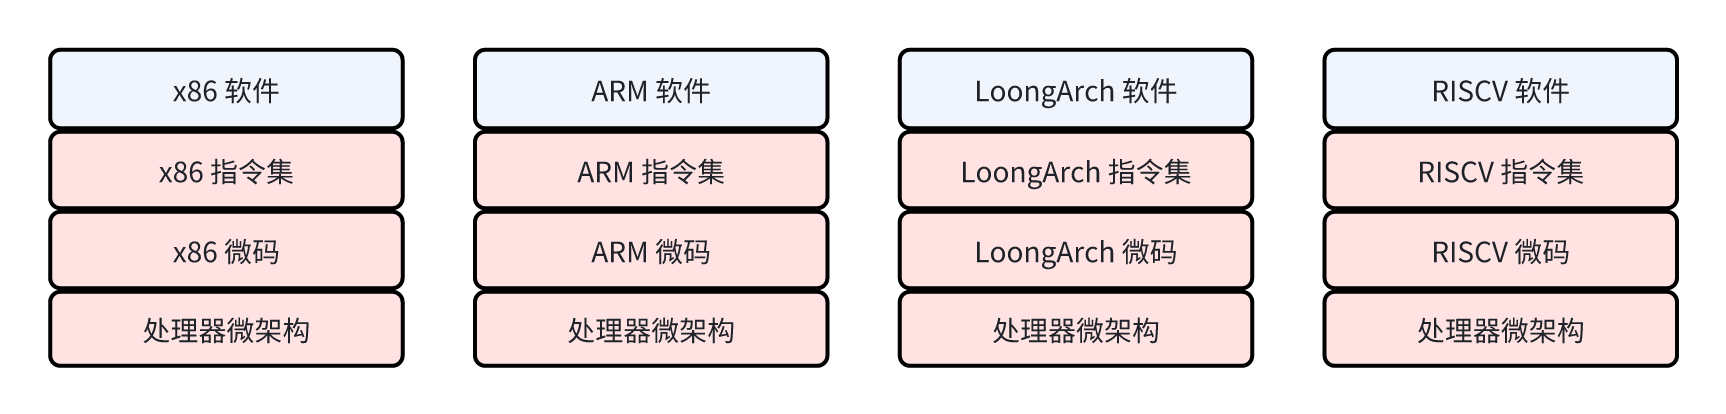
\includegraphics[width=1\linewidth]{./feishuImage/allCPU_arch.png}
    \caption{不同指令集CPU的架构图,图中白色为软件层,红色为硬件层,并忽略了操作系统,这不是本文研究重点。\protect\footnotemark}
    \label{img:allCPU_arch}
  \end{figure}

\footnotetext{ARM, LoongArch, RISCV 等精简指令集架构(RISC)的CPU,内部可以实现微码层,也可以不实现,根据具体CPU微架构实现而不同。}

如图\ref{img:allCPU_arch}所示,同一套软件源代码需要针对不同的指令集进行编译才能在不同架构的CPU上运行\footnotemark。

\footnotetext{这里主要关注C/C++等底层语言,对于Java等支持跨平台运行的语言,也需要Java虚拟机对不同指令集平台进行编译适配。}

    而中国国产CPU的多样性导致了指令集的碎片化,增加了应用程序在不同架构间迁移和适配的复杂性。存在的问题包括:
    \begin{itemize}
    \item \textbf{适配和迁移负担:} 不同架构间的适配和迁移需要大量人力和物力资源。
    
    \item \textbf{历史兼容包袱:} 不同指令集的历史兼容包袱使得跨架构的兼容性复杂。
    
    \item \textbf{编译与源代码的限制:} 古老软件无源代码,只能通过翻译运行以适应新的指令集。
    
    \item \textbf{操作系统支持的挑战:} 操作系统厂商需要投入更多资源以支持不同架构。
    \end{itemize}

\section{二进制翻译器性能问题}
目前,二进制翻译技术是解决指令集兼容性问题的主要方法。

\begin{figure}[h]
    \centering
    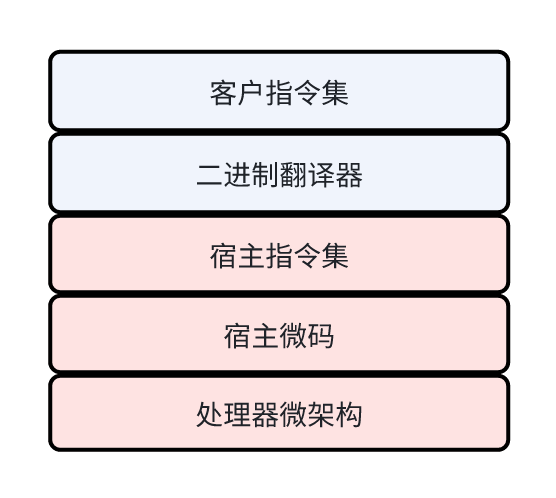
\includegraphics[width=0.3\linewidth]{./feishuImage/BT_arch.png}
    \caption{二进制翻译器架构图,能在宿主指令集机器上运行客户程序。}
    \label{img:BT_arch}
  \end{figure}

如图\ref{img:BT_arch} 二进制翻译技术能够将一个指令集(称为客户指令集)上的二进制程序翻译到另一种指令集(称为宿主指令集)上执行,分为系统级和用户级二进制翻译。系统级翻译涉及整个操作系统,而用户级翻译主要处理用户程序。用户级翻译由于不需要模拟特权态和物理内存,因此性能更高,在软件生态迁移中更为常见,在后文中提及的二进制翻译器默认为用户级二进制翻译器。

% \section{二进制翻译器性能问题}
现有的开源二进制翻译器性能
\footnote{
    目前工业界和学术界对二进制翻译的性能有着默认统一的定义:同一份测试程序的源码用相同编译参数,编译到客户指令集和宿主指令集,得到两份二进制文件$B_g$和$B_h$。
    在硬件平台用二进制翻译运行客户程序$B_g$的时间记为$T_{bt}$,在同一硬件平台直接运行宿主程序$B_h$的时间记为$T_h$。
    二进制翻译的性能则为翻译运行时间除以原生运行时间$\frac{T_{bt}}{T_h}$。
}
相对较低,例如QEMU\cite{bellardQEMUFastPortable2005}虽然支持多架构应用,但在翻译运行SPEC CPU 2017\cite{SPECCPU2017}程序时候,仅有约10\%的性能。商业二进制翻译器也存在性能损失,
如苹果的Rosetta2\cite{RosettaTranslationEnvironment, RunningIntelBinaries}、
华为的ExaGear\cite{KunPengExaGear}、
和龙芯的LATX\cite{LoongArchEnv2022, LoongArch2023},
性能仅达到原生运行的70\%左右,并且仅能保证单一指令集翻译到单一指令集,并不通用,多架构支持较为困难。这直接影响了软件生态迁移的流畅度和成功性。

% \section{多架构软硬协同二进制翻译的需求}
\section{本文的主要工作及贡献}

为了解决\textbf{指令集碎片化}和\textbf{二进制翻译器性能}问题,迫切需要多架构软硬协同的二进制翻译技术。这项技术的关键目标是在同一套硬件下实现多指令集的共存,为软件提供更好的跨平台兼容性和性能表现。

这种技术的优势在于:

1. \textbf{打破指令集边界,消除应用迁移成本:} 应用程序无需适配和迁移至特定指令集,可直接在同一套硬件上运行,降低了软件开发和维护的复杂性。

2. \textbf{硬件对外暴露微码,规避X86等授权问题:} 通过在硬件层面暴露微码,技术在一定程度上规避了X86等架构的授权问题,提高了国产CPU的自主性。

3. \textbf{软件维护历史兼容,微码迭代优化:} 作为软件层面的核心组件,二进制翻译器维护历史兼容性并实现微码迭代优化,确保不同架构的硬件在不同历史时期的应用中保持高效运行。

如图\ref{img:my_arch}所示,本文提出了一种多架构软硬协同的二进制翻译技术,通过在硬件层面支持一套融合微码,为软件层面的二进制翻译器提供更好的性能和兼容性。这项技术可降低软件开发和维护的复杂性,弥合不同指令集的生态差异,对中国国产CPU的发展具有重要意义。


\begin{figure}[h]
    \centering
    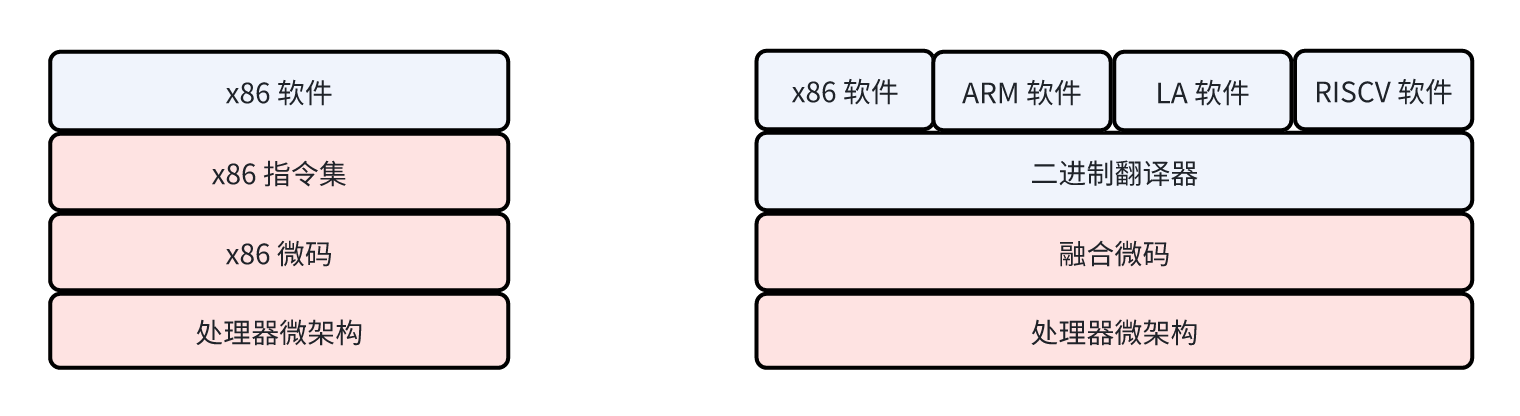
\includegraphics[width=1\linewidth]{./feishuImage/my_arch.png}
    \caption{多架构软硬协同的二进制翻译架构图,硬件仅对外暴露微码,软件层面的二进制翻译器可以实现多架构的支持,性能接近原生运行性能。}
    \label{img:my_arch}
  \end{figure}




\section{论文的组织结构}
\chapter{相关工作}\label{chap:related_work}

本章主要介绍二进制翻译的相关工作,包括著名的几款软件二进制翻译器,如QEMU、Rosetta2、ExaGear、LATX等,
并对二进制翻译器的性能开销进行分析,发现间接跳转的性能开销以及指令集语义差异是二进制翻译器性能的主要瓶颈。
接下来介绍软硬协同二进制翻译器的相关工作,包括超长指令字兼容和指令集扩展,但仍有一定局限性。
为了解决间接跳转和指令集语义差异的问题,引出了复杂指令集x86处理器的微码缓存的概念,为微译器的设计提供了设计思路。

\section{软件二进制翻译器}

软件二进制翻译器是一种通过软件实现的二进制翻译器,
它对硬件改动较小,能够在不同的硬件平台上运行,因此具有更好的可移植性和灵活性。
本节主要介绍一款开源的用户态二进制翻译器QEMU,以及三款商用级的用户态二进制翻译器,包括苹果公司的Rosetta2、华为公司的ExaGear、龙芯公司的LATX。
其中Rosetta2和LATX也有硬件支持,但主要还是依赖软件实现,因此归类为软件二进制翻译器。

\subsection{QEMU}

QEMU是一个广泛使用的开源多平台二进制翻译框架,特别在云计算环境中,它常和KVM一起使用,提供了一种高效的虚拟化解决方案。
QEMU同时支持系统态翻译和用户态翻译,本文主要关注用户态翻译部分,它允许在一个主机操作系统上模拟另一个操作系统的应用程序。

QEMU也同时支持多种架构,包括x86、ARM、RISC-V等,使其成为开发跨平台应用程序的理想工具, 也可用于软件开发、测试以及安全研究。
如图\ref{img:qemu_arch},它通过将不同指令集的机器代码翻译成中间语言(IR,Intermediate Representation),再将IR翻译成宿主指令集,实现跨架构的兼容性。
这种设计使得QEMU能够处理多种指令集,为用户提供了一定的灵活性。然而,QEMU的性能仅能达到原生性能的10\%,
这主要归因于双层翻译(客户代码翻译到IR,IR翻译到宿主代码)的性能损失以及Helper函数模拟浮点和向量指令的性能开销\cite{deflater}。

\begin{figure}[!htbp]
  \centering
  \includegraphics[width=0.6\linewidth]{./image/qemu-IR.pdf}
  \caption{QEMU二进制翻译器架构图,能在宿主指令集机器上运行多种客户程序。}
  \label{img:qemu_arch}
\end{figure}

基于QEMU的优化主要旨在提高其性能和执行效率,例如中间代码优化\cite{LiNan2021}、基本块链接优化\cite{Hong2012HQEMUAM}、缓存管理\cite{FengYue2010}、Helper函数优化\cite{Wang2021}等。
以下给出两个优化示例,包括HQEMU的多线程并行翻译和执行,以及寄存器分配的优化。

HQEMU\cite{Hong2012HQEMUAM}是一个基于QEMU和LLVM构建的多线程和可重定向动态二进制翻译器。
这个项目的目标是通过利用多核处理器的并行处理能力来减轻DBT的开销,同时允许更复杂的优化技术的应用。
HQEMU通过在不同的线程上分别运行QEMU翻译器和LLVM优化器,从而实现了这一目标。
在一系列基准测试中,比如SPEC CPU2006,HQEMU在x86到x86-64的模拟中,相比于原始的QEMU性能提高了2.4倍至4倍。

在动态二进制翻译中,寄存器分配是提高翻译代码执行效率的关键。原始的QEMU在许多宿主机上将所有目标寄存器映射到内存,并仅将少数临时变量存储在宿主寄存器中。
这种方法并没有考虑相邻指令之间的依赖关系,导致即使在执行前一个指令时已经将一个客户寄存器的值加载到临时变量中,执行下一个指令时也需要再次从内存中重新加载该值。
为了解决这个问题,\cite{Hong2012HQEMUAM}提出了一个优化方法,其在两个或更多相邻指令执行中有效利用了临时变量,
从而减少了对内存的不必要访问。通过这种优化,基准测试显示可以实现10\%到20\%的速度提升。

尽管以上优化示例展示了通过改进QEMU的翻译过程和内部机制,可以提升QEMU的效率和性能,
但是改进后的性能仍然仅相当于原生性能的一小部分,这在一些对性能要求较高的应用场景下显得不够可用。


\subsection{Rosetta2}

Rosetta2 是苹果公司开发的商用二进制翻译系统,
通过支持预先编译(AOT)和即时编译(JIT)两种模式实现动静结合翻译,
预先翻译对性能影响大的代码,并把翻译后代码保存在磁盘上,而对于需要动态解析的代码,采用即时编译的方式进行翻译。
Rosetta2 主要针对64位的x86\_64指令集进行翻译,以适配苹果M1等ARM64处理器的架构。

Rosetta2 的核心目标是保证MacOS上的软件能够在ARM架构下运行,这要求对系统调用进行转换,以匹配基于ARM的MacOS版本。
由于x86和ARM指令集都采用小端法(little-endian),这简化了指令翻译过程,避免了复杂的字节序反转操作。
这一点与苹果过去从PowerPC(大端法,big-endian)切换到x86的过程不同,后者在转换时面临更多的挑战。

然而,x86(强内存序)与ARM(弱内存序)在内存一致性模型上的差异可能导致多线程软件运行结果出现差异,这是模拟x86的一个主要挑战\cite{Risotto}。
苹果通过在芯片内部额外实现一个Intel版本的强内存TSO模型,并通过后门开关在运行Rosetta2时切换到该内存模型,解决了这一问题。
硬件支持的内存模型有效的降低来并发程序翻译的性能开销,提高了Rosetta2的性能。

\subsection{ExaGear}

ExaGear是华为公司开发的动态二进制翻译软件,专为在基于自研的ARM鲲鹏服务器上运行而设计。
ARM服务器由于其能效比优势,逐渐在数据中心中得到广泛应用,但是由于软件生态的限制,一些只有x86版本的软件无法在ARM服务器上运行。
ExaGear通过将x86应用程序翻译为ARM指令集,使得这些软件能够在ARM服务器上运行。

ExaGear通过修改Linux的binfmt\_misc组件,使得系统能够识别并使用ExaGear作为x86应用程序的解析器,实现了在安装过程中的高效集成。
ExaGear主要包括两个关键组件:指令翻译引擎和x86运行环境。指令翻译引擎充当x86应用程序与ARM架构服务器之间的中间件,实现了在x86应用程序启动时的实时翻译功能。
这一过程对用户完全透明,确保了用户体验的一致性。x86运行环境为x86应用程序提供了必要的标准库、实用程序和配置文件,构建了一个完整的运行时环境。
此外ExaGear还通过Trace优化技术来减少分支数目,进而改善内存布局和局部性,减少间接跳转查找过程\cite{LvYandong2021}。

\subsection{LATX}

龙芯二进制翻译器(LATX)是龙芯公司开发的一款动态二进制翻译软件,用于在龙芯处理器(LoongArch架构)上运行x86架构的应用程序。
结合LATX和Wine\cite{amstadt1994wine}(一 个 操 作 系 统 API翻译软件,它可以用Linux的系统调用来模拟实现Windows的系统调用,从而实现在Linux/ x86上运行Windows/x86的应用程序),
用户可以在龙芯处理器上运行大量的x86应用程序,包括Windows应用程序,例如微信、WPS、部分游戏等。

后文\ref{sec:isa_extension}节会讲解,通过添加龙芯二进制翻译扩展指令(LBT),LATX能生成出更接近x86语义的宿主指令,而无需用多条指令模拟。
此外,LATX 也添加了各类优化措施,例如x86 EFLAGS延迟计算、基本块链接、跨基本款反馈优化等,更多细节可以参考胡起的硕士论文\cite{HuQi2023}。

表\ref{tab:BTs} 对本节提到的4个主流的二进制翻译器进行了总结。

\begin{table}[!htbp]
  \centering
  \caption{主流二进制翻译器}
  \label{tab:BTs}
    \begin{tabular}{llll}
    \rowcolor[HTML]{FBE5D6} 
    二进制翻译器    & 公司   & 客户平台           & 宿主平台           \\
    QEMU      & 开源项目 & x86,ARM,RISC-V等 & x86,ARM,RISC-V等  \\
    ExaGear   & 华为   & x86            & ARM            \\
    Rosetta2  & 苹果   & x86            & ARM            \\
    LoongArch & 龙芯   & x86            & LoongArch      
    \end{tabular}
    \end{table}

\section{软件二进制翻译的性能开销分析}\label{sec:bt_overhead_all}

\subsection{理论分析}\label{sec:bt_overhead}

在进行性能分析之前,我们可以先对二进制翻译器的性能开销进行理论分析。
如图\ref{img:bt_overhead},二进制翻译的性能开销主要分为两类:指令集语义差异和二进制翻译器机制的开销。

\begin{figure}[!htbp]
  \centering
  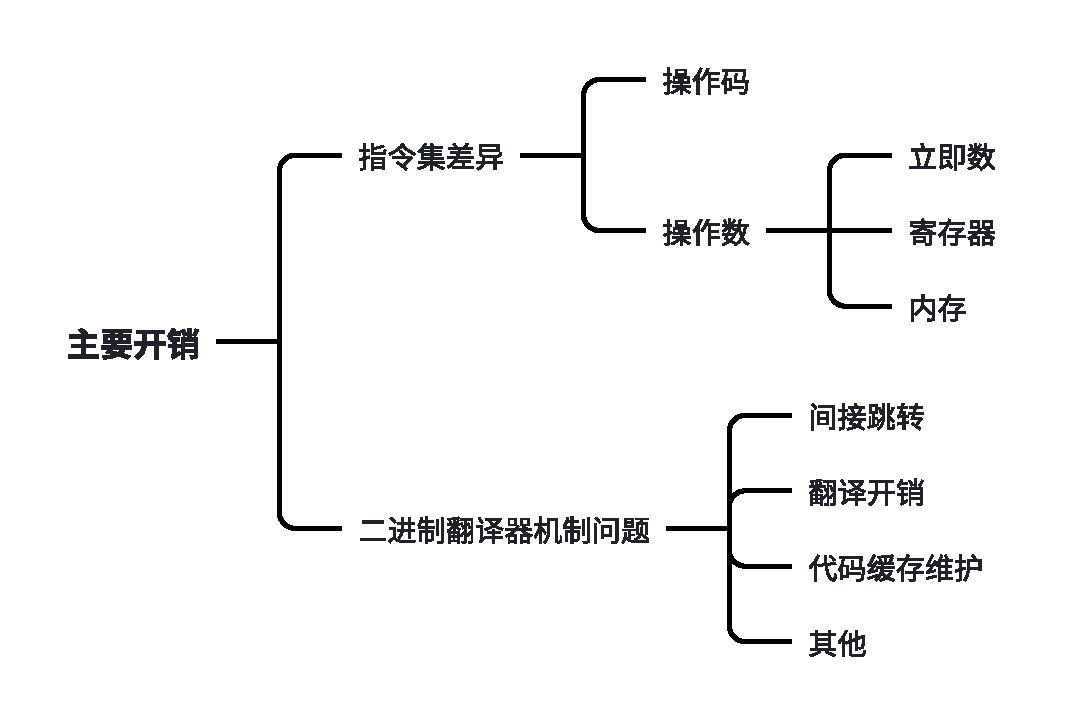
\includegraphics[width=0.7\linewidth]{./feishuImage/overhead_all.pdf}
  \caption{二进制翻译器的性能开销分析。}
  \label{img:bt_overhead}
\end{figure}

指令集是计算机软件和硬件交互的接口,是定义了计算机的操作和数据的格式的一种规范。
指令包括操作码和操作数,操作码是指令的功能码,操作数是指令的操作对象。其中操作数按照操作对象可以分为立即数、寄存器、内存等。
\begin{itemize}
\item 操作码不同导致一条客户指令翻译成多条宿主指令。
\item 如果客户指令的立即数范围大于宿主指令的立即数范围,那么需要额外的指令来加载立即数。
\item 如果客户指令的寄存器数量大于宿主指令的寄存器数量,那么需要额外的指令来保存和恢复寄存器,也称为寄存器溢出。
\item 如果客户指令的内存访问模式复杂,那么需要额外的指令来计算内存地址。
\end{itemize}

而二进制翻译器机制的开销主要包括:
\begin{itemize}
\item 间接跳转的性能开销:如图\ref{img:indirect_jump},间接跳转是指在程序运行时,通过读取寄存器的值来决定跳转到哪个地址。这种跳转方式在静态翻译时无法确定,因此需要在运行时查询哈希表来确定跳转地址。
\item 翻译开销:翻译开销是指动态二进制翻译器在翻译客户指令时产生的性能开销。这种开销主要包括指令翻译、基本块优化、基本块链接等。
\item 代码缓存维护: 二进制翻译器需要维护一个软件的代码缓存,用于存储翻译后的宿主指令。当缓存满时,需要进行缓存替换产生开销。
\end{itemize}

\begin{figure}[!htbp]
  \centering
  \includegraphics[width=0.8\linewidth]{./image/indirect_jump.pdf}
  \caption{间接跳转开销,由于翻译后的代码地址发生了非线性偏移,间接跳转的目标地址只能在运行时查询哈希表获取。}
  \label{img:indirect_jump}
\end{figure}

\subsection{实验分析}

上一节提到的商用级用户级二进制翻译器,包括苹果公司的Rosetta2、华为公司的ExaGear、龙芯公司的LATX,
在运行SPEC2017基准测试时,根据\ref{eq:bt_performance}公式,得到的翻译性能分别为67.2\%、72.7\%和60\%,
距离原生性能100\%还有较大的差距,为此希望通过实验分析找出二进制翻译器的性能瓶颈。


\begin{figure}[!htbp]
  \centering
  \rotatebox{90}{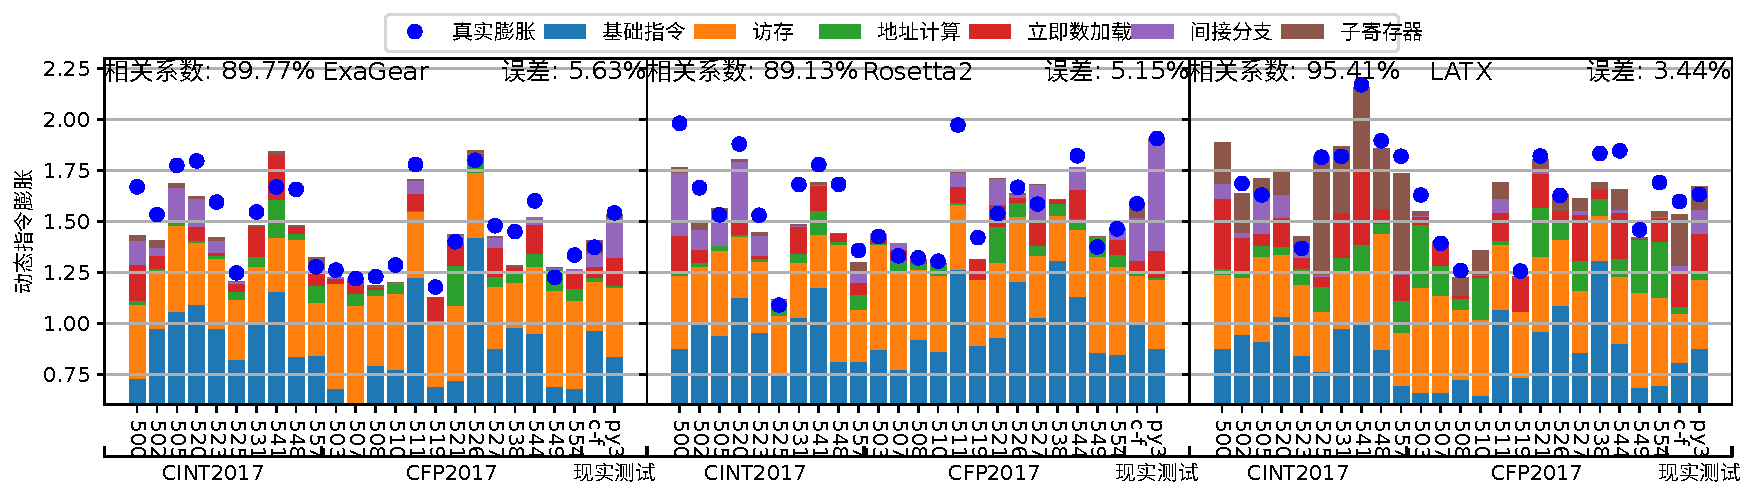
\includegraphics[width=\textheight,height=\textwidth,keepaspectratio]{./plot_pdf/insts_inflt_breakdown_2017.pdf}}
  \caption{各个二进制翻译器在运行SPEC2017的指令膨胀来源分析图\cite{deflater}。}
  \label{img:insts_inflt_breakdown_2017}
\end{figure}

根据本团队之前完成的一项工作\cite{deflater},基于如下两个前提,使用使用指令膨胀率来分析二进制翻译器的性能开销。
\begin{enumerate}
\item  为了保证客户程序的精确异常,二进制翻译器不会做指令重排这样的激进优化,即保持指令的顺序不变。
\item  主流二进制翻译器在运行SPEC 2017这类运算密集型的基准测试时,98\%的时间都在执行生成的宿主指令上,翻译过程的性能开销是可以忽略不计。
\end{enumerate}

指令膨胀率是指,每条客户指令平均翻译出的宿主指令数,是一个大于1的小数,计算方式参考\ref{eq:insts_inflt}。
举例来说,一条x86的add指令可能翻译成LoongArch的load指令和一个add指令,那么这条x86 add指令的膨胀率就是2。
对所有的客户指令的膨胀率求加权平均值,权重为客户指令的动态执行次数,即得到了整个程序的指令膨胀率
(为了说明简单,忽略了基本块内指令的优化)。
假设所有指令执行时间相同,那么膨胀了多少倍,程序的执行时间就会变长多少倍。
事实上,不同指令的执行时间是不同的,但可以大致通过指令膨胀率来估计程序的性能开销。
指令膨胀率越高,翻译后的程序要执行的指令数越多,执行时间越长,性能越低。即便多发射处理器能在单拍内执行多条指令,缓解更多指令带来的性能开销,
但根据测试数据,指令膨胀率和性能下降值保持正相关\cite{deflater}。

\begin{equation}
  \text{总体膨胀} = \frac{\text{生成的宿主指令数}}{\text{客户指令数}} \\
  = \frac{\sum_i \text{指令频次}_i \times \text{指令膨胀率}_i}{\sum_i \text{指令频次}_i}
  \label{eq:insts_inflt}
\end{equation}

如图\ref{img:insts_inflt_breakdown_2017},
测量并模拟了3款商用级二进制翻译器(ExaGear、Rosetta2、LATX)在运行SPEC2017的指令膨胀率,模拟误差在5\%以内。
注意这三款翻译器都是复杂指令集(x86)到精简指令集(ARM/ LoongArch)的翻译器,这两类指令集语义差异较大,因此指令膨胀率较高。
图中\ref{img:insts_inflt_breakdown_2017}蓝色的点表示测量的真实膨胀率,而分解成不同颜色的柱状图表示模拟的膨胀率来源。
根据指令膨胀率的来源,主要将开销分成了5类:


%latex 使用1. 2. 3. 来编号
\begin{enumerate}
  \item \textbf{指令集间操作码差异:} 不同指令集的操作码差异引起Eflags计算等操作的额外指令翻译,增加了指令膨胀率。此外LoongArch对于子寄存器默认符号扩展,x86/ARM默认零扩展。对应图\ref{img:insts_inflt_breakdown_2017}中\textcolor{Sepia}{\textbf{棕色}}部分。
  
  \item \textbf{操作数据模式不同:} 复杂指令集(x86)可以直接访问内存,而其他精简指令集只能操作寄存器,导致操作数模式不同。对应图\ref{img:insts_inflt_breakdown_2017}中\textcolor{orange}{\textbf{橙色}}部分。
  
  \item \textbf{地址计算不同:} 复杂地址计算方式(x86)与其他指令集的简单计算方式导致在翻译时需要额外指令。例如x86计算地址$addr = base + index * scale +disp$; 其他的大多为$addr = base + offset$。 对应图\ref{img:insts_inflt_breakdown_2017}中\textcolor{green}{\textbf{绿色}}部分。
  
  \item \textbf{立即数加载:} x86是变长指令集,支持编码64位立即数和32位地址偏移;而其他指令集均为定长指令集,立即数的编码空间有限。在翻译一条带有长立即数的指令时,需要额外的访存指令(从内存加载长立即数)或者是多条立即数加载指令(多个短立即数拼接成一个长立即数)。对应图\ref{img:insts_inflt_breakdown_2017}中\textcolor{red}{\textbf{红色}}部分。
  
  \item \textbf{间接跳转:} 客户指令地址到宿主指令地址是非线性的,而间接跳转的目标地址在运行时才能知道,需要额外的几条指令查询间接跳转哈希表,导致性能开销。对应图\ref{img:insts_inflt_breakdown_2017}中\textcolor{Purple}{\textbf{紫色}}部分。
  
\end{enumerate}

以上五类主要开销也对应于上一节\ref{sec:bt_overhead}理论分析的内容:
前4个属于指令集语义差异(操作数据模式不同也属于复杂指令集和精简指令集的差异,也可归为操作码不同),而间接跳转属于二进制翻译机制问题。
由于x86\_64通用寄存器只有16个,少于ARM/LoongArch的32个通用寄存器,所有没有寄存器溢出产生的开销。
而翻译开销和代码缓存维护的开销在现代高性能二进制翻译器中也是可以忽略不计的。

以上这5类主要开销很难通过软件优化来解决,接下来将介绍软硬协同二进制翻译器的相关工作。

\section{软硬协同二进制翻译器}

指令集作为软件和硬件沟通的桥梁,设计初衷是让软件和硬件设计解耦,使得软件开发者不需要关心硬件的细节,只需要关心软件的逻辑。
而二进制翻译器则是一种将不同指令集之间的桥梁,它可以将不同指令集的二进制代码翻译为目标指令集的二进制代码,从而实现不同指令集之间的兼容。
从设计层次来看,二进制翻译器相对指令集更加靠近硬件层,因此添加硬件支持的软硬协同二进制翻译器是一个比较自然的选择。

此外,二进制翻译器一般应用于生态迁移,在处理器厂商推出新型处理器时,为了保持对旧软件的兼容性,或者引入其他指令集已有的繁荣生态,需要引入二进制翻译器。
处理器厂商也有动力在新型处理器中添加硬件支持,以提高二进制翻译器的性能,减少软件兼容的性能开销。
本节主要介绍两个代表性的软硬协同二进制翻译器,分别是Transmeta公司的超长指令字兼容和龙芯公司的指令集扩展技术。

\subsection{超长指令字}

在处理器设计早期,由于当时的硬件晶体管资源有限,难以硬件发掘指令集并行性,因此超长指令字(Very Long Instruction Word, VLIW)技术应运而生。
超长指令字技术通过软件来发掘指令级并行性,将多条指令打包成一条超长指令字,从而提高指令级并行性,提高处理器的性能。
Transmeta公司推出的Crusoe处理器就是一种基于超长指令字的处理器,其宣称在性能和功耗方面都优于同期的x86处理器\cite{dehnertTransmetaCodeMorphing2003}。

但由于初期超长指令字技术的复杂性和软件开发者对于超长指令字的不熟悉,导致超长指令字生态并不繁荣,
因此Transmeta公司配套推出了软件上的代码转换器(Code Morphing Software, CMS),通过软硬协同的方式实现了对x86指令集的兼容。
Transmeta的CMS充当了翻译器和优化器的角色,使得基于非x86的VLIW处理器能够执行x86二进制代码。
还提供了一个动态优化的执行环境,能够在运行时对代码进行优化,从而提高执行效率和能耗性能\cite{dehnertTransmetaCodeMorphing2003}。

如图\ref{img:transmeta_arch}所示,代码转换器将从程序接收到的x86汇编代码指令翻译成微处理器的本机指令(超长指令字)。
通过这种方式,Crusoe 也可以模拟其他指令集架构,例如Crusoe 也能将字节码翻译为其本机指令集中的指令来执行 Java 字节码。

\begin{figure}[!htbp]
    \centering
    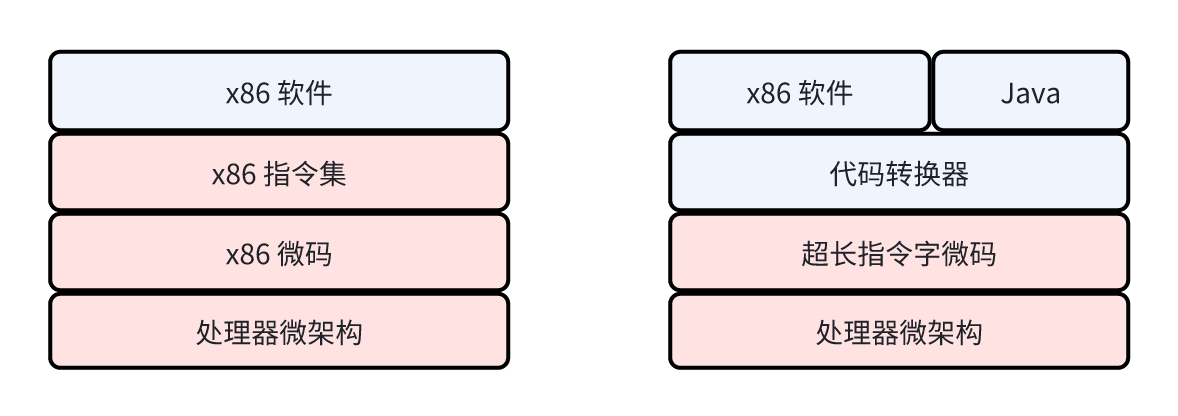
\includegraphics[width=0.8\linewidth]{./feishuImage/transmeta_arch.png}
    \caption{Transmeta架构图,在超长指令字处理器上实现兼容x86的指令集,并支持JAVA程序。}
    \label{img:transmeta_arch}
  \end{figure}
这种架构有如下特点:

\begin{itemize}
\item 架构兼容性与灵活性:Transmeta从初代128位VLIW处理器到第二代的256位VLIW处理器,都能通过软件翻译器保持软件兼容。
\item 解释与翻译配合:冷客户代码通过解释执行,热代码通过翻译执行,提高了执行效率。
\item 精确异常处理:Transmeta在硬件中引入了一套提交和回滚机制,当发生异常时,配合软件翻译器回滚,能够保证异常处理的精确性。
\end{itemize}

尽管Transmeta公司提出了许多创新的技术,但并未在市场上取得成功,最终于2007年退出处理器市场。
随着半导体工艺进步,处理器的晶体管资源变得丰富,基于硬件的乱序执行技术逐渐成熟,已经能够用硬件发掘指令级并行性,
超长指令字技术的优势逐渐减弱,超长指令字技术的发展也逐渐停滞。
但Transmeta公司在多架构兼容性方面的工作提供了宝贵的经验,成为软硬结合二进制翻译器的重要先驱者。

\subsection{指令集扩展}\label{sec:isa_extension}

客户和宿主指令集语义差异是二进制翻译器性能的主要瓶颈之一,为了解决这个问题,在宿主指令集中添加指令集扩展来接近客户指令集的语义是一种常见的解决办法。
例如龙芯公司在LoongArch指令中添加的二进制翻译扩展指令(Loongson Binary Translation, LBT)\cite{LoongArch2023}。

龙芯早期使用MIPS指令集,并添加了便于x86和ARM二进制翻译的一系列自定义指令集,例如对x86 EFLAGS的支持、对X87浮点指令的支持、非对齐访存的支持等,形成了LoongISA\cite{LoongISA}。
但由于MIPS中用户定义指令(UDI)槽位有限,导致了LoongISA的指令集扩展受限,
所以在2020年龙芯公司发布了全新的、自主可控的、支持更多指令集扩展的LoongArch架构\cite{LoongArch2023}。
并从3A5000开始,龙芯处理器开始支持LoongArch架构,并配套使用LATX二进制翻译器进行x86应用程序的翻译。
LoongArch指令集中同样增加了对二进制翻译的扩展指令集,称为LBT(Loongson Binary Translation)指令集,用于支持x86、ARM、MIPS的二进制翻译。
LBT扩展指令集与LATX软件配合使用,可以实现更高效的二进制翻译,提高了龙芯处理器的软件兼容性。

指令集扩展虽然能够接近客户指令集的语义,但这样会增加宿主指令集的复杂度,更加剧了指令集的历史包袱,同时添加指令集扩展也难以支持多种指令集的兼容。


% \section{x86 微码缓存的相关工作}
\section{x86处理器微码缓存}\label{sec:complex_isa}

x86 微码缓存是为了在 x86 CPU 后端实现超标量乱序执行并降低译码功耗而引入的关键组件\cite{solomonMicrooperationCachePower2001},如图\ref{img:front_end_ucache}。以下是关于 x86 微码缓存的主要工作和设计特点:

\begin{figure}[!htbp]
  \centering
  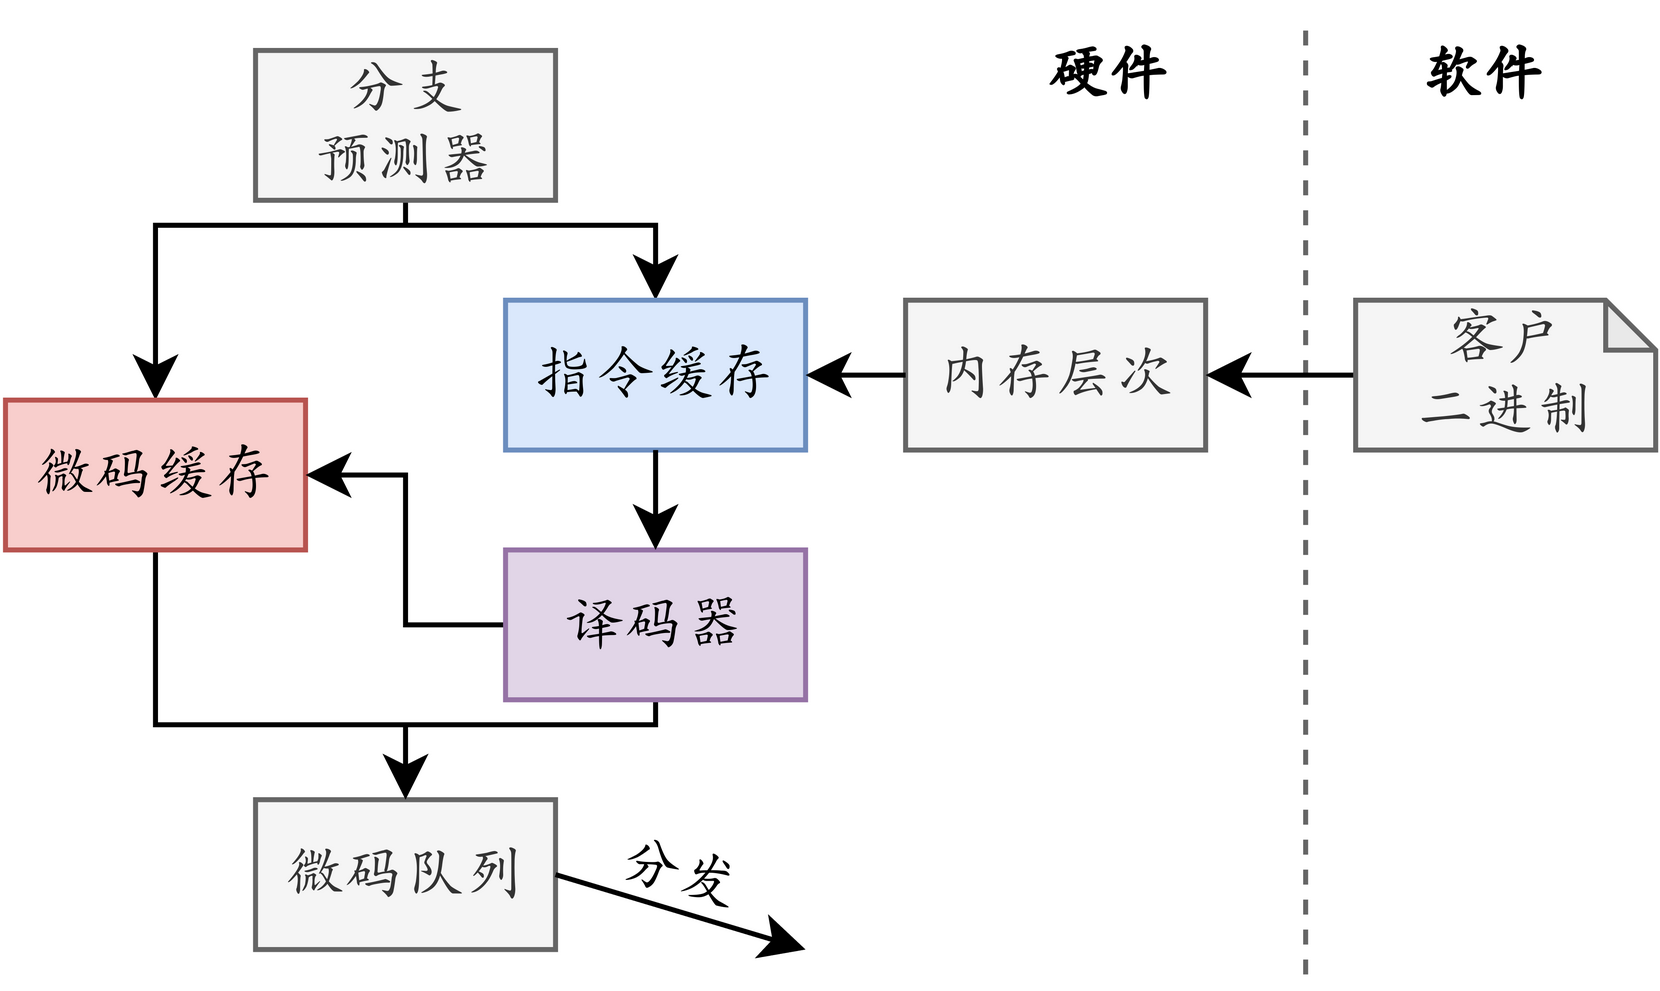
\includegraphics[width=0.6\linewidth]{./image/front_end_ucache.pdf}
  \caption{x86处理器前端架构图,包括指令缓存和微码缓存。
  如果微码已缓存则直接使用;如果微码未缓存则从指令缓存中取得指令,进行译码并存入微码缓存中。}
  \label{img:front_end_ucache}
\end{figure}

\subsection{微码缓存介绍}

1. \textbf{微码与超标量乱序执行的关系:}

为了实现超标量乱序执行,x86 CPU 后端需要将复杂的变长x86指令转换成类RISC格式的定长微码。
微码的引入简化了指令集的关系,降低了CPU后端设计复杂度,使得指令能在后端能够更高效地乱序执行。

2. \textbf{微码缓存的引入:}

为了降低译码能耗、提高性能,研究者们引入了微码缓存,用于存储已经译码过的微码。
如果这条指令已经译码过,就直接从微码缓存中读取微码,而不需要再次译码。
\cite{solomonMicrooperationCachePower2001}论文中指出,在标准测试集中,
微码缓存能消除75\%的指令译码,在多媒体应用中,这个比例甚至高达90\%。
对于Intel P6处理器来说,能节省10\%左右的整机功耗。

3. \textbf{查询与缓存机制:}

具体而言,在CPU的前端,指令缓存和微码缓存是分开的,如图\ref{img:front_end_ucache}。
在前端译码阶段,系统会首先查询微码缓存,检查是否已经缓存了当前指令的微码。
如果微码已经在缓存中,CPU 就直接读取微码并发射到后端执行。
如果微码未缓存,系统则从指令缓存中取得指令,进行译码,并将译码结果存入微码缓存中,注意一个指令缓存行可能生成多个微码缓存行。

4. \textbf{缓存组织形式:}

\begin{figure}[!htbp]
  \centering
  \includegraphics[width=0.8\linewidth]{./image/ucache.pdf}
  \caption{微码缓存的组织形式}
  \label{img:ucache}
\end{figure}

微码缓存的组织形式与指令缓存有所区别。指令缓存的地址被分为标记、索引和块偏移三部分,而微码缓存的地址被分为标记、索引两部分,其中地址低位的块偏移也是标记的一部分。
这是因为一条指令会被译码为多条数量不定的微码,原本的块偏移无法唯一标识一条微码。
多条指令组成的指令基本块(以控制流指令结尾)译码成的多条微码,会尽可能放在一个微码行中,然后用指令基本块的首地址来索引这个微码行。
同时一个指令缓存行产生的多个微码缓存行会放在同一个微码缓存组中,当需要刷新这一行指令缓存时, 可以方便的通过索引找到对应的微码缓存行进行刷新。
如图\ref{img:ucache},指令地址首先通过索引找到对应的微码组,然后通过标记找到对应的微码行。
微码行开头有元信息存储有关这个微码行的信息,例如微码数量、立即数数量等。接下来读出对应的微码,发射到后端执行。

由于x86是变长指令集,微码是定长指令集,如果x86指令中有长立即数,会放在微码行的最后。
所以微码行中除了存入微码外,还会在最后存储立即数,见图\ref{img:ucache_line}。
微码和立即数是相向生长的,微码从前往后,立即数从后往前,如果相遇,说明微码行已满,需要分配新的微码行。

\begin{figure}[!htbp]
  \centering
  
\includegraphics[width=0.8\linewidth]{./image/ucache_line.pdf}
  \caption{微码缓存一行的内容}
  \label{img:ucache_line}
\end{figure}

5. \textbf{微码缓存行的结束条件:}

微码指令会尽可能填满一个微码缓存行,但是当满足如下3个条件之一时,会结束当前微码缓存行的填充\cite{solomonMicrooperationCachePower2001}:
\begin{enumerate}
  \item 遇到指令缓存行的结尾:一行指令缓存可能对应多行微码缓存,这意味着当遇到指令缓存行结尾时,
  微码缓存会截断这一行,这样当一行指令缓存行需要刷新时,容易找到对应的多行微码缓存行进行刷新。
  \item 遇到控制流指令并预测会跳转:当遇到控制流指令时,微码缓存会截断这一行,确保每个微码缓存行只包含一个基本块的微码。
  \item 微码缓存行已满:当微码缓存行中微码或者立即数填满一行时,会结束当前微码缓存行的填充。
\end{enumerate}

此外,为了保证一条宏码对应的多条微码一起提交,在后端重排序缓冲区(ROB)中需要添加对应的标志位,标记这些微码是一起提交的。
(例如一条复杂的x86指令可能会翻译成多条微码,这些微码在后端原子化提交,保证精确异常处理)。

\begin{figure}[!htbp]
  \centering
  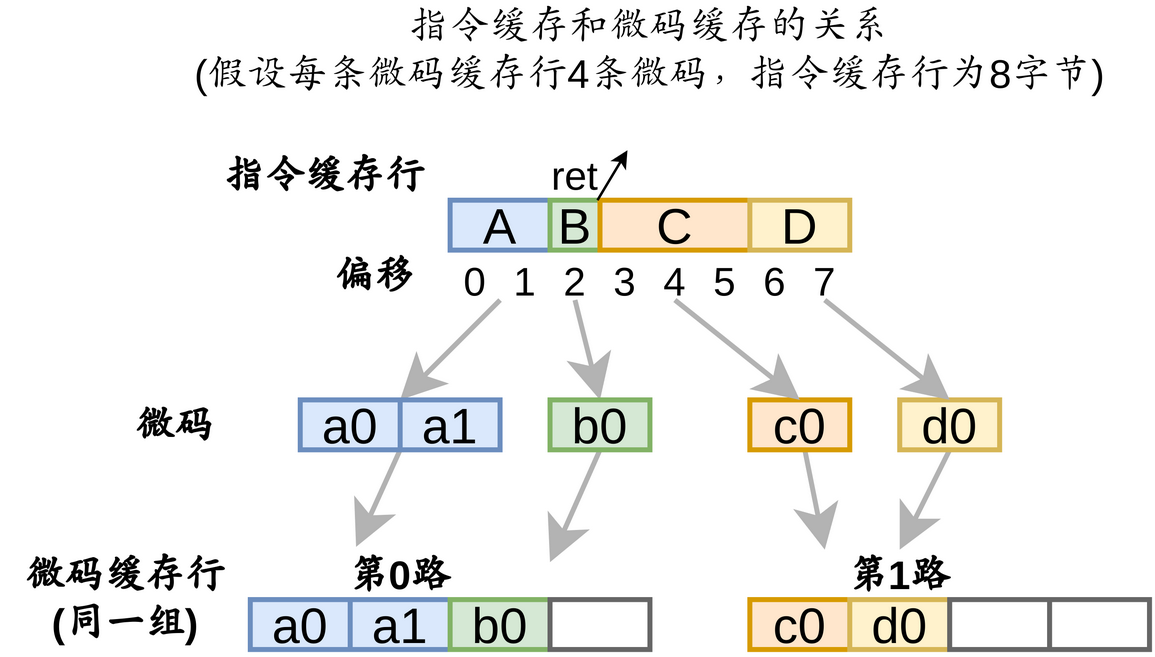
\includegraphics[width=0.8\linewidth]{./image/IC-to-UC.pdf}
  \caption{指令缓存和微码缓存关系}
  \label{img:IC_to_UC}
\end{figure}

如图\ref{img:IC_to_UC}给出了一行指令缓存对应多行微码缓存的示例(这里的微码行忽略了立即数的存储)。
假设指令缓存行为8字节,存储了A、B、C、D四条指令,分别长度为2、1、3、2字节,微码缓存行最多能存储4条微码。
4条指令译码得到的微码分别为a0、a1、b0、c0、d0。
则微码缓存行1存储了a0、a1、b0,微码缓存行2存储了c0、d0。
本来c0是可以存储在微码缓存行1中的,但是由于B指令是控制流ret指令,满足结束条件2,所以微码缓存行1结束,c0存储在微码缓存行2中。
此外微码缓存行1和微码缓存行2是存放在同一个微码缓存组中不同路上的,意味着它们的索引相同,但是标记不同。
加入这一行指令缓存行需要被刷新,可以通过索引找到这两行微码缓存行一起刷新,而无需刷新整个微码缓存,保证了指令缓存行和微码缓存行的一致性。

x86 微码缓存的引入和优化为 x86 架构的超标量乱序执行提供了重要支持,使得 CPU 在执行 x86 指令集时能够更加高效地利用硬件资源,提高整体性能。

% \subsection{微码与二进制翻译相似性}

% 二进制翻译会在软件层将客户指令翻译成宿主指令,
% 而x86处理器前端在硬件层将x86指令翻译成微码。
% 二进制翻译中使用代码缓存存储翻译后的宿主指令,而x86处理器使用微码缓存存储译码后的微码。
% 二进制翻译可以添加指令集扩展来缩小和客户指令语义差异,而x86处理器的微码也可以不断修改来适应新的指令集扩展。

% 而对于二进制翻译中间接跳转的复杂处理,本质上是由于客户地址到宿主地址的非线性映射导致的,需要额外的指令来查询哈希表。
% 但微码缓

% \section{本章小结}

% 本文采用了硬件辅助的策略。其中,一些关键的工作包括:

% 1. 融合微码以缩小指令集语义差距: 针对指令集间操作码差异、操作数据模式不同以及地址计算不同等问题,通过融合微码的方式,减小不同指令集之间的语义差距,从而降低翻译的开销。

% 2. 微码缓存的思路应用: 针对立即数加载和间接跳转的性能开销,借鉴了x86微码缓存的思想,将立即数放入微码缓存行中直接加载,用微码缓存直接查询非线性的地址空间映射,消除这两类开销。

% 本章首先介绍了软件二进制翻译器
\chapter{微译器设计与实现}\label{chap:MUT}

前文\ref{sec:bt_overhead_all}通过分析发现二进制翻译器的主要开销来源于指令集语义差异和间接跳转开销。

指令集语义差异的一种常见的解决办法是在宿主指令集中添加指令集扩展,来接近客户指令集的语义,例如LoongArch指令中添加的二进制翻译扩展指令(Loongson Binary Translation, LBT)\cite{LoongArch2023}。
但这样会增加宿主指令集的复杂度,更加剧了指令集的历史包袱,同时添加指令集扩展也难以支持多种指令集的兼容。
本课题从X86处理器定义的微码指令集中得到启发,微码是一种内部指令集,不对外暴露给用户和编译器,并且可以随着处理器的演进而不断迭代优化,不需要考虑历史兼容包袱。

通过定义一套\textbf{融合微码},作为一种内部指令集,包含各个指令集的并集,对外不暴露给用户,而是通过二进制翻译器将客户指令翻译为融合微码指令,从而实现多指令集的兼容。
在这个层面上,二进制翻译器类似于一个软件译码器,将客户指令翻译为融合微码指令,而CPU则类似于一个虚拟机,执行融合微码指令。
由于X86授权问题,直接做一个硬件译码器对外支持X86指令集是不现实的,因此通过软硬协同的方式,软件的二进制翻译器将客户指令翻译为融合微码指令,再由硬件执行融合微码指令。

而对于间接跳转开销,X86的微码缓存天然的就能解决这个问题,因为硬件上的微码缓存维护好了X86指令地址和微码指令地址的映射关系,
可以通过简单的查询缓存访问到微码指令地址,
而不需要软件上复杂的哈希表查询逻辑,这样可以大大减少间接跳转的开销。
因此参考X86的微码缓存,本课题提出了一种\textbf{翻译缓存}的概念,用于存储预翻译的融合微码指令集。
% 一条X86指令译码为多条微码指令,这个和一条宿主指令翻译为多条客户指令类似,都是一种一对多的关系。

总结起来,通过借鉴X86微码和微码缓存的概念,本团队提出了一种多架构软硬协同的二进制翻译技术——\textbf{微译器},
通过\textbf{融合微码}缩小了指令集语义差异,
通过\textbf{翻译缓存}来消除间接跳转开销,提高了二进制翻译器的性能。

\section{微译器整体架构}

\begin{figure}[!htbp]
  \centering
  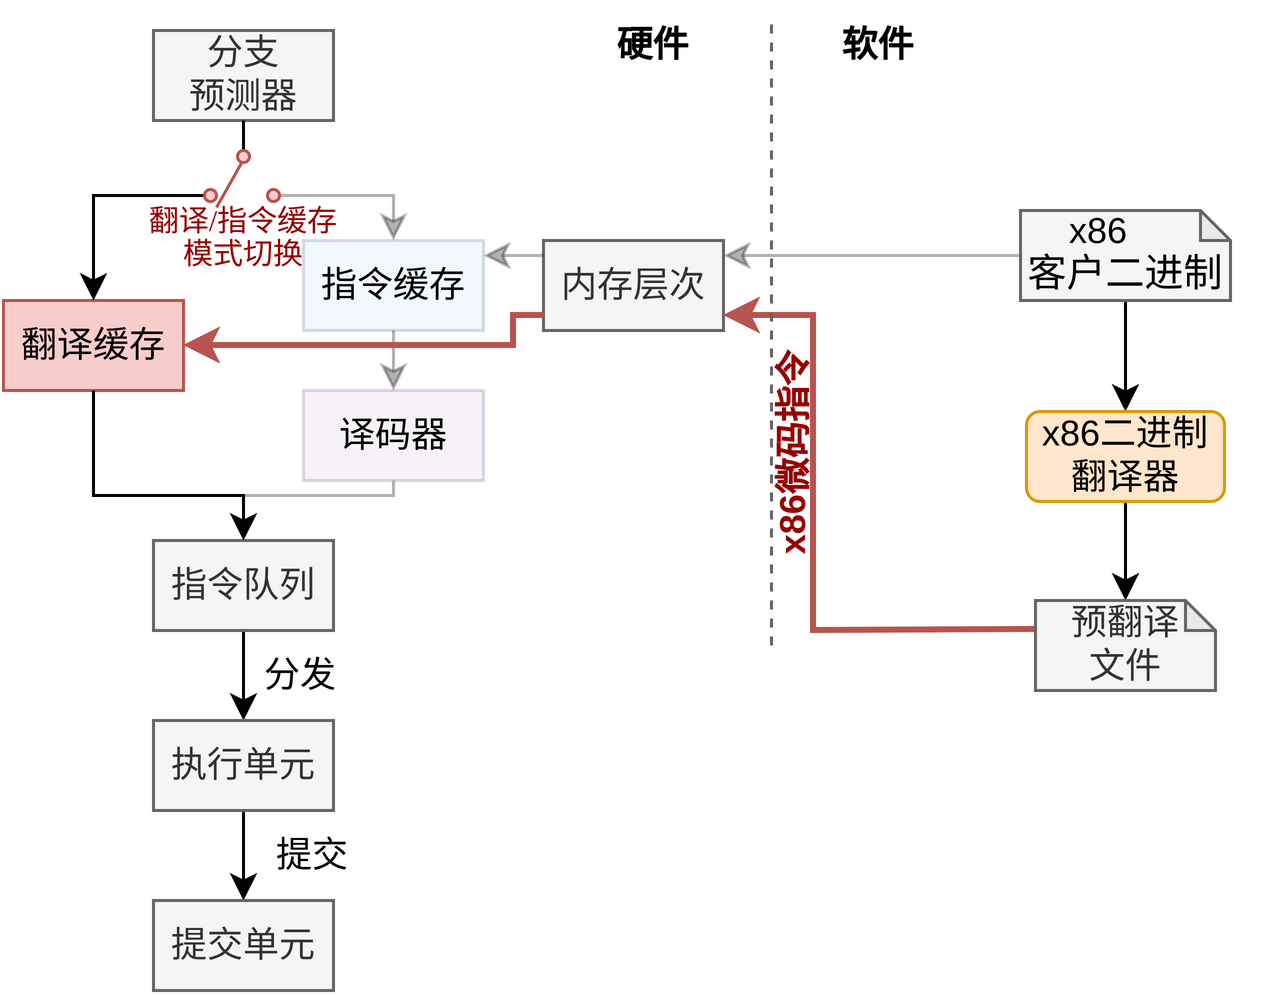
\includegraphics[width=0.8\linewidth]{./image/front_end_transutor.pdf}
  \caption{微译器整体架构图}
  \label{img:front_end_transutor}
\end{figure}

如图\ref{img:front_end_transutor}展示了微译器的整体架构,相对于传统的X86处理器前端图\ref{img:front_end_ucache},微译器在硬件侧和软件侧都做了一些改动。

% \subsection{硬件部分}

在硬件部分,引入了\textbf{翻译缓存}(Translation Cache),该缓存作为一级缓存负责存储预翻译的微码指令集,替代了原本的微码缓存。
翻译缓存的每行组织形式和微码缓存类似,都是前面部分存放微码指令(这里为融合微码指令,下一节详细介绍),
后面存放立即数,微码指令和立即数相向生长,中间可能有空洞,产生新的开销,后文会提出对应的优化方案。

此外与传统微码架构不同,微码缓存数据是直接来源于CPU和指令缓存,通过硬件译码器进行译码并存入微码缓存中;
而翻译缓存通过软件的二进制翻译“译码”,透过内存层次(从内存加载到L3 Cache, 再到L2Cache, 最后到微码缓存)进行填充,
取代了传统的指令缓存和译码器的角色。
在传统X86架构下,取指部件会同时查询指令缓存和微码缓存;
而在微译器架构下,取指部件仅查询翻译缓存,硬件的译码器被软件的二进制翻译器取代。
为了兼容传统的X86处理器模式,添加了一个模式切换逻辑,可以切换回使用硬件译码器进行译码,这样可以在不改变原有X86处理器的基础上实现微译器的功能。
后文默认使用软件二进制翻译器进行译码,也就是翻译缓存的方式。

% \subsection{软件部分}

在软件部分,引入了静态和动态二进制翻译器。
程序首先通过静态二进制翻译器被翻译成融合微码指令,并被写入预翻译文件,存储在硬盘中。
在客户程序执行阶段,预翻译文件被加载到内存中,程序计数器被设置为客户程序的入口。
取指部件从翻译缓存中取指,若翻译缓存或内存层次命中,则从翻译缓存取指,发送到处理器后端执行,不断取指执行。
若翻译缓存和内存层次均未命中(例如存在自修改代码等),说明客户指令还未翻译,此时会调用动态二进制翻译器进行实时翻译,
并将翻译结果写入翻译缓存,再取指执行。

接下来详细介绍微译器各个组成部分的设计与实现,包括融合微码、翻译缓存、预翻译文件、二进制翻译器。

\section{融合微码}\label{sec:tisa}
本节详细介绍重要的一个概念——融合微码。“融合”代表它能融合了多种指令集的特征,
包括X86和RISCV,未来还可以支持ARM,MIPS等其他指令集,
或许叫统一微码也更好理解。但融合并非简单的把所有指令集简单拼接就好,这会造成指令集冗余,挤占有限的编码空间。
而是需要对各个指令集的特征进行分析,找到共性,抽象出一种更加简洁的指令集,这就是融合微码的设计思想。

“微码”这个名字主要由于它在翻译缓存中的组织形式和传统的X86微码缓存组织形式类似,并且更像是不同指令集的更低级表现形式;
此外目前第一代的融合微码是在原有的Gem5 X86微码上扩充的,
所以便于理解仍然保留融合微码的名字。

但事实上,融合微码有很大特征很像一个“RISC指令集”。
由于融合微码指令是需要存储在磁盘中的,并不像传统X86微码只是作为一个“暂时指令”存在于CPU运行期间,
所以融合微码指令需要像普通指令集一样进行\textbf{编码},
二进制翻译器把指令\textbf{编码}为定长的融合微码指令,并存储于磁盘中。
CPU再从磁盘中加载融合微码指令,\textbf{解码}为CPU识别的信息,这一阶段也叫“译码阶段”。
因此从这个角度来说,加上指令定长、只能操作寄存器、指令间关系被简化等特征,融合微码很像一个普通的“RISC指令集”。
因此融合微码类似传统指令集概念,也是有编码空间的概念。

\section{翻译缓存}\label{sec:tcache}

本节讲解翻译缓存的设计与实现,翻译缓存是微译器的核心组件,用于存储预翻译的融合微码指令集。

翻译缓存的结构整体和微码缓存类似,但是有一些细节上的差异,在此详细介绍翻译缓存行的组织形式,
重点关注元信息和数据部分,其余的标签、有效位等部分和普通的一级缓存类似。
一篇关于微码缓存的专利\cite{uopPatent}中提到了微码缓存的一行设置为74byte。
而本文设计的翻译缓存行的大小为64字节,结构类似图\ref{img:ucache_line},但是元信息部分有所不同。

\begin{figure}[!htbp]
  \centering
  \includegraphics[width=1\linewidth]{./image/tcache_line.pdf}
  \caption{翻译缓存行组织形式}
  \label{img:tcache_line}
\end{figure}

如图\ref{img:tcache_line},展示了翻译缓存行的组织形式,主要对元信息部分进行了详细介绍。
翻译缓存行的大小为64字节,
前16字节存放元信息,元信息细分为两部分,第一字节存放这一行的元信息,包括这一行是否有效,对应多少条宏码指令(这里的宏码就是客户指令,用宏码是为了和微码做对应)。
接下来15字节存放每条宏码的元信息,最多可以存15条宏码指令,宏码指令元信息包括宏码指令的长度(X86指令是变长指令,存储长度来索引到下一条X86指令地址),这条宏码生成的微码数量。
最后的48字节存放微码指令和立即数,微码指令和立即数都是定长的,单位为4字节。微码指令和立即数相向生长,中间可能有空洞。

存储行信息、微码指令、立即数是十分必要的,而存储宏指令元信息是为了支持二进制翻译器中精确异常处理。
精确异常处理是指在异常发生时,这条宏指令之前的所有指令都已经执行完毕,这条宏指令之后的所有指令都没有执行。
因此需要把一条宏指令对应的几条微码看做一个整体,可以乱序执行,但是在提交阶段需要保证这几条微码指令是原子提交的。
这样就能保证精确异常处理,这也是二进制翻译器必须要支持的功能。
因此在宏指令元信息中,需要存储一条宏指令对应的微码数量信息,而宏码长度信息则为了取到下一行微码缓存行。


\section{预翻译文件}\label{sec:aot}

本节讲解预翻译文件(Ahead-of-Time, AOT)的设计与实现,预翻译文件是存储预翻译的融合微码指令集的文件,是静态二进制翻译器的输出。

预翻译文件的设计思想在于,尽可能多的存储所有可能用到的融合微码指令,减少动态二进制翻译的开销。
由于融合微码和普通指令在一级缓存中寻址模式不同,普通指令能根据行内偏移直接访问到指令,而融合微码只能根据行内第一条指令的地址访问到整行指令(在\ref{sec:complex_isa}小节有提到)。
也就是说,融合微码只能以一个微码行(一个基本块)为单位进行访问,而不能以一个微码指令为单位进行访问。
如果出现了跳转到一个微码行的中间位置,那么就需要重新翻译这个微码行,这样会增加额外的开销。
对于传统的X86处理器模式,这个开销是很小的,因为是硬件来译码并填充到微码缓存中,只需要2拍左右;
而对于微译器架构,这个开销就会很大,因为需要调用软件的二进制翻译器进行实时翻译,可能需要上百拍的开销,这样的开销是无法接受的。
因此提出了\textbf{重复存储}的概念,即存储任意一个地址开始的融合微码指令,这样就能保证在跳转到任意一个地址时,都能从预翻译文件中加载对应的融合微码指令。


\section{二进制翻译器}

软件端的二进制翻译器分为静态二进制翻译器和动态二进制翻译器,静态二进制翻译器用于将客户程序翻译为融合微码指令,并存储在预翻译文件中;
动态二进制翻译器用于在翻译缓存未命中时实时翻译客户指令。

首先介绍静态二进制翻译器,它有如下3个设计目标:
\begin{enumerate}
  \item 可扩展性强:能够方便支持多种指令集的翻译。
  \item 代码发现性强:能够发现更多的二进制代码进行翻译,减少动态二进制翻译的介入。
  \item 可维护性强:能够方便的维护和更新翻译器。
\end{enumerate}

\begin{figure}[!htbp]
  \centering
  \includegraphics[width=1\linewidth]{./image/mut_bt.pdf}
  \caption{静态二进制翻译器架构图}
  \label{img:mut_bt}
\end{figure}

因此在实现上,如图\ref{img:mut_bt},尽可能的将翻译器的功能模块化,分为代码发现模块、反汇编模块、翻译模块、提交模块。
代码发现模块用于尽可能的发现更多的二进制代码,例如通过符号表、字符串表等信息发现更多的代码;
反汇编模块用于将ELF文件中的二进制代码转换为汇编代码;
翻译模块用于将汇编代码翻译为融合微码指令;
提交模块用于将翻译后的融合微码指令组织成翻译缓存行的形式,写入预翻译文件。

此外将架构相关的代码和架构无关的代码分开,架构相关的代码只有翻译模块,架构无关的代码主要是代码发现模块、反汇编模块和提交模块。
这样只需要添加新的翻译模块,就能够支持新的指令集的翻译,而不需要修改其他模块的代码。

最后会希望尽可能复用现有的工具,例如LLVM objdump工具用于代码发现,这样能够减少二进制翻译器的实现难度,提高开发效率;
使用capstone工具用于反汇编,这样能够减少反汇编的实现难度,提高反汇编的准确性。
此外选用的LLVM objdump 和capstone工具都天然支持多种指令集,这样能够方便未来支持多种指令集的翻译。


而对于动态二进制翻译器,它的基本功能是在翻译缓存未命中时实时翻译客户指令,它和静态二进制翻译器的功能类似,
只是触发时机不同,因此我们可以复用静态二进制翻译器的代码,只需要添加一个触发机制即可。
它有两个触发机制,一个是代码发现没有发现的代码,需要实时翻译;一个是由于自修改代码等原因,翻译缓存行失效,需要实时翻译。
具体在硬件上,当翻译缓存行失效时,会触发例外(类似缺页异常),这时会调用动态二进制翻译器进行实时翻译,将翻译结果写入翻译缓存。

% \section{微译器的优势}

% \subsection{消除间接跳转开销}

% \begin{figure}[!htbp]
%   \centering
%   \includegraphics[width=1\linewidth]{./image/indirect_jump_transutor.pdf}
%   \caption{静态二进制翻译器架构图}
%   \label{img:mut_bt}
% \end{figure}

% \subsection{消除立即数膨胀开销}

% \begin{figure}[!htbp]
%   \centering
%   \includegraphics[width=1\linewidth]{./image/mut_bt.pdf}
%   \caption{静态二进制翻译器架构图}
%   \label{img:mut_bt}
% \end{figure}
\chapter{RISCV指令支持}\label{chap:RISCV}

设计一套高效完备的融合微码“指令集”是一个长期的工程,这不是本文研究重点。
为了快速验证微译器的实际效果,同时减少“指令集设计”产生的额外性能影响,
因此目前我们的融合微码是基于在原本的Gem5 X86微码上扩充的,并谨慎的添加了部分RISCV指令,
如图\ref{img:TISA},由于X86指令默认符号扩展,而RISCV指令同时支持符号扩展和零扩展,
为了尽可能实现一条RISCV指令翻译成一条融合微码指令,所以需要添加适当的“零扩展”微码指令。

\begin{figure}[h]
  \centering
  \includegraphics[width=0.8\linewidth]{./image/TISA.pdf}
  \caption{指令翻译到融合微码过程,X86 add 和RISCV add 指令都翻译成融合微码add指令,
  而lbu(加载字节并无符合扩展)指令,需要额外添加lbu 微码指令。}
  \label{img:TISA}
\end{figure}

\section{RISCV指令翻译}

目前已经完成所有的RISCV指令(包括IMAFDC指令集)到融合微码的翻译。

\begin{itemize}
  \item 整数指令(I): 主要包括运算指令、逻辑指令、跳转指令、访存指令等。大部分复用X86微码,访存指令等需要额外添加新的微码。

  \item 乘除法指令(M):主要包括乘法、除法、取余等指令。大部分复用X86微码。

  \item 原子指令(A):包括原子加法、原子比较等指令。由于目前尚未实现多线程支持,
  原子加法指令被翻译为一条普通load+加法指令+一条store指令。

  \item 浮点指令(F,D):包括单精度浮点F 和双精度浮点D指令。大部分复用X86微码,出于简洁考虑,对于特殊的舍入模式暂未考虑和X86的差异。

  \item 压缩指令(C):为了压缩指令长度,把常用的4字节指令替换为2字节长度的压缩指令。尽可能把翻译得到的微码也编码为2字节。

\end{itemize}

累积统计数目如下:原本X86指令共有数千条,X86微码也有500余条。
为了添加272条RISCV指令,我们并没有简单添加272条微码指令,
而只是添加了41条整数相关指令,10条浮点相关指令,累计添加51条微码指令。

\section{处理ABI差异}
%介绍什么是ABI, 从而引出RISCV和X86的ABI差异。而我们的项目需要把RISCV的ABI转换成X86的ABI。
ABI全称为Aplication Binary Interface,是程序和硬件的统一接口,不同指令集的ABI也是不同的,
在二进制翻译系统中需要维护这种差异性,保证程序运行的正确性。
ABI包括内容比较多,其中主要的包括系统调用传参、初始化栈等问题,本节介绍微译器项目是如何处理ABI差异的。


\subsection{系统调用差异}

如表\ref{tab:syscall}所示,X86和RISCV的系统调用号和参数传递方式的差异。
X86的系统调用号存储在rax寄存器中,返回值也存储在rax寄存器中,参数传递方式为rdi, rsi, rdx, r10, r8, r9。
而RISCV的系统调用号存储在a7寄存器中,返回值存储在a0寄存器中,参数传递方式为a0, a1, a2, a3, a4, a5。
因此我们需要在RISCV的二进制翻译器中,将RISCV的系统调用号和参数传递方式转换成X86的系统调用号和参数传递方式。

参数传递的差异可以通过把X86的参数寄存器和RISCV的参数寄存器映射到相同的微码寄存器即可,如表\ref{tab:reg_map}所示,
所有的黄色寄存器就是6个参数传递寄存器。系统调用号差异同理也可解决。


\begin{table}[]
  \centering
  \caption{
    X86和RISCV的系统调用号和参数传递方式的差异。
  }
  \label{tab:syscall}
  \begin{tabular}{llllllllll}
  \rowcolor[HTML]{FFCC67} 
  \cellcolor[HTML]{FBE5D6}指令集 & \cellcolor[HTML]{FBE5D6}系统调用号 & \cellcolor[HTML]{FBE5D6}返回值 & 参数1 & 参数2 & 参数3 & 参数4 & 参数5 & 参数6 & 其他参数 \\
  X86                         & rax                           & rax                         & rdi & rsi & rdx & r10 & r8  & r9  & 栈传递  \\
  RISCV                       & a7                            & a0                          & a0  & a1  & a2  & a3  & a4  & a5  & 栈传递 
  \end{tabular}
  \end{table}


\subsection{寄存器映射表}

寄存器映射一直是二进制翻译中一个重要的研究课题。
如表\ref{tab:reg_map}所示,展示了X86和RISCV映射到微码的的寄存器映射表。
对于X86寄存器映射到微码寄存器较为容易,因为X86只有16个通用整数寄存器,而微码我们定义了32个通用寄存器,
所以只需要把X86寄存器固定映射到前16个通用寄存器即可,还可以把一些常用的寄存器
(例如AH,BH等子寄存器和段寄存器)映射到后面的寄存器中,还可用一些寄存器作为临时寄存器供二进制翻译器使用。

但是对于RISCV映射到微码方案,由于RISCV本身就有32个通用寄存器,固定映射到32个微码寄存器后,
就没有额外的临时寄存器供二进制翻译器使用了。对于微译器项目,得益于软硬件协同设计的基本原则,
我们额外添加了两个微码寄存器作为临时寄存器,
这两个寄存器只对二进制翻译器可见,不对RISCV应用程序可见,类似于X86“段寄存器”,属于特殊寄存器。



\begin{table}[]
  \centering
  \caption{
    X86和RISCV的寄存器映射表。
  }
  \label{tab:reg_map}
  \begin{tabular}{|
    >{\columncolor[HTML]{FFCCC9}}l |l|l|
    >{\columncolor[HTML]{FFCCC9}}l |
    >{\columncolor[HTML]{FFFFFF}}l |
    >{\columncolor[HTML]{FFFFFF}}l |
    >{\columncolor[HTML]{FFCCC9}}l |
    >{\columncolor[HTML]{FFFFFF}}l |
    >{\columncolor[HTML]{FFFFFF}}l |
    >{\columncolor[HTML]{FFCCC9}}l |
    >{\columncolor[HTML]{FFFFFF}}l |
    >{\columncolor[HTML]{FFFFFF}}l |}
    \hline
    \cellcolor[HTML]{FBE5D6}微码 & \cellcolor[HTML]{FBE5D6}X86 & \cellcolor[HTML]{FBE5D6}RISCV & \cellcolor[HTML]{FBE5D6}微码 & \cellcolor[HTML]{FBE5D6}X86 & \cellcolor[HTML]{FBE5D6}RISCV & \cellcolor[HTML]{FBE5D6}微码 & \cellcolor[HTML]{FBE5D6}X86 & \cellcolor[HTML]{FBE5D6}RISCV & \cellcolor[HTML]{FBE5D6}微码 & \cellcolor[HTML]{FBE5D6}X86 & \cellcolor[HTML]{FBE5D6}RISCV \\ \hline
    0                          & \cellcolor[HTML]{FFFC9E}RAX & \cellcolor[HTML]{FFFC9E}A7    & 8                          & \cellcolor[HTML]{FFFC9E}R8  & \cellcolor[HTML]{FFFC9E}A4    & 16                         & T0                          & Zero                          & 24                         & CH                          & S8                            \\ \hline
    1                          & \cellcolor[HTML]{FFFFFF}RCX & \cellcolor[HTML]{FFFFFF}TP    & 9                          & \cellcolor[HTML]{FFFC9E}R9  & \cellcolor[HTML]{FFFC9E}A5    & 17                         & T1                          & RA                            & 25                         & DH                          & S9                            \\ \hline
    2                          & \cellcolor[HTML]{FFFC9E}RDX & \cellcolor[HTML]{FFFC9E}A2    & 10                         & \cellcolor[HTML]{FFFC9E}R10 & \cellcolor[HTML]{FFFC9E}A3    & 18                         & T2                          & S2                            & 26                         & ES                          & S10                           \\ \hline
    3                          & \cellcolor[HTML]{FFFFFF}RBX & \cellcolor[HTML]{FFFFFF}GP    & 11                         & R11                         & A6                            & 19                         & T3                          & S3                            & 27                         & CS                          & S11                           \\ \hline
    4                          & \cellcolor[HTML]{FFFFFF}RSP & \cellcolor[HTML]{FFFFFF}SP    & 12                         & R12                         & T1                            & 20                         & T4                          & S4                            & 28                         & SS                          & T3                            \\ \hline
    5                          & \cellcolor[HTML]{FFFFFF}RBP & \cellcolor[HTML]{FFFFFF}T0    & 13                         & R13                         & T2                            & 21                         & T5                          & S5                            & 29                         & DS                          & T4                            \\ \hline
    6                          & \cellcolor[HTML]{FFFC9E}RSI & \cellcolor[HTML]{FFFC9E}A1    & 14                         & R14                         & S0                            & 22                         & AH                          & S6                            & 30                         & FS                          & T5                            \\ \hline
    7                          & \cellcolor[HTML]{FFFC9E}RDI & \cellcolor[HTML]{FFFC9E}A0    & 15                         & R15                         & S1                            & 23                         & BH                          & S7                            & 31                         & GS                          & T6                            \\ \hline
    \end{tabular}
    \end{table}

% \subsection{栈的初始化}
% 由于我们目前关注于用户态二进制翻译器,不太涉及系统态指令的翻译和处理操作系统等概念,
% 但是当加载运行不同指令集的程序时,在libc库眼中,操作系统已经准备好了这个程序的初始化栈等信息,例如argc,argv参数、
% 环境变量指针等,对于X86和RISCV程序,这个初始化栈是不同的,需要不同的处理
\chapter{RISC-V微译器优化方案}\label{chap:Opt}

前文\ref{sec:tcache}中提到了翻译缓存的引入能消除间接跳转的开销,
上一节\ref{sec:RISC-V-translation}中添加适当的融合微码指令能缩小指令集语义差异,共同提升二进制翻译器的性能。
然而,RISC-V微译器的引入也会带来一些新的问题,产生新的性能瓶颈,本节将首先分析RISC-V微译器的开销来源,然后
针对这些问题提出一些优化方案,从而减缓这些性能瓶颈,进一步提升性能。




\section{RISC-V微译器开销来源}
RISC-V微译器的主要开销来源于磁盘、内存、缓存三个方面,前两者来源于预翻译文件中\textbf{重复存储}机制,后者来源于翻译缓存的\textbf{存储效率}问题。
重复存储机制是为了减少动态二进制翻译的开销,提高性能,但是会增加磁盘和内存的开销;
存储效率问题是由于翻译缓存行的固定长度,导致存储效率较低,缓存缺失率较高,进而影响性能。
本小节主要分析重复存储机制,下一小节将分析存储效率问题并给出优化方案。

预翻译文件的作用和可执行文件(Linux中为ELF格式文件)类似,是存储程序的二进制指令的文件格式,处理器会从预翻译文件中加载融合微码指令集,进而译码执行。
预翻译文件的数据段和ELF文件数据段相同,但是由于重复存储机制,代码段相对于ELF文件的代码段会膨胀64倍(64为翻译缓存行长度),接下来会举例介绍预翻译文件的代码段格式。

\begin{figure}[!htbp]
  \centering
  \includegraphics[width=1\linewidth]{./image/aot_format.pdf}
  \bicaption{\enspace 预翻译文件格式}{\enspace The format of the Ahead-of-Time file}
  \fignote{A、B、C、D为客户指令,a0、b0、c0、d0为翻译出的融合微码指令,由于重复存储,会存储a0-b0-c0-d0、b0-c0-d0、c0-d0、d0这
  四行融合微码指令,并填充对齐。}
  \label{img:aot_format}
\end{figure}

如图\ref{img:aot_format},展示了预翻译文件的代码段格式,为了简单起见,假设图中的指令缓存行大小为8字节,包含4条客户指令A、B、C、D,
起始地址分别为0x0、0x2、0x3、0x6,
生成的融合微码指令为a0、b0、c0、d0。
对应的预翻译文件会有8行,每行长度为64字节(相对于ELF文件膨胀了64倍)。
第0行(地址0x0)存储A指令开始的所有融合微码指令a0、b0、c0、d0;
第2行(地址0x80)存储B指令开始的所有融合微码指令b0、c0、d0;
第3行(地址0xC0)存储C指令开始的所有融合微码指令c0、d0;
第6行(地址0x180)存储D指令开始的所有融合微码指令d0。
其余的第1、4、5、7行都是空行,用于填充对齐。
能看出来,ELF 文件中代码地址和预翻译文件中代码地址是线性映射关系,只需要简单的地址映射就能找到对应的融合微码指令,地址关系如下:

\begin{equation}
Addr_{AOT} = Base +  Addr_{ELF} \times 64 
\end{equation}

再回顾一下,为何需要\textbf{重复存储}融合微码指令呢?这是因为可能有指令跳转到一行的中间位置(例如跳转到指令C),
这样就需要从预翻译文件中加载C指令开始的融合微码指令。
如果只存储A指令开始的融合微码指令,那么在跳转到C指令时,就需要重新翻译C指令开始的融合微码指令,这样会增加额外的开销,
这个开销包括调用动态二进制翻译器进行实时翻译、翻译缓存的填充等,需要数百拍才能完成,因此为了减少这个开销,需要重复存储融合微码指令。


\textbf{重复存储}办法本质上是一种用空间换时间的策略,通过增加预翻译文件的大小,减少了动态二进制翻译的开销,提高了性能。
虽然文件代码段膨胀了64倍,但目前主流的SPEC 2017程序的代码段大小在几十MB,这样的膨胀对于现代存储设备来说并不是很大的开销。
而对于内存来说,预翻译文件中有大量的空行,可以通过压缩算法进行透明压缩,减少内存占用,Linux中的zswap技术就是这样的一种技术。
对于多级缓存来说,只有被取到的缓存行才会被加载到缓存中,未被取到的缓存行不会被加载到缓存中,例如图\ref{img:aot_format}中可能只有第一行被取到,其他行不会被加载到缓存中。


\section{翻译缓存优化}

本文设计中,翻译缓存是和指令缓存同级的(或者说,是用于\textbf{替换}指令缓存的),用于存放融合微码指令。
如果翻译缓存大小和指令缓存大小相同,总行数相同,那么一行中存放的指令数量越多,缓存的总指令数量就越多,
缓存缺失率就会越低,性能就会越好,
因此翻译缓存的存储效率对性能影响较大,
存储效率的定义如公式\ref{eq:store_efficiency}所示。

% 存储效率公式
\begin{equation} \label{eq:store_efficiency}
  \text{存储效率} = \frac{\text{实际存放的指令数量}}{\text{缓存行能存储的最大指令数量}}
\end{equation}


如前文\ref{sec:tcache}所述,翻译缓存的每行组织形式和微码缓存类似,都是前面部分存放微码指令,后面存放立即数,微码指令和立即数相向生长,中间可能有\textbf{空洞}。
此外对于64字节长度的翻译缓存行,本文还设计了一个16字节长的元信息部分,用于存储一些额外的信息,如指令类型、指令长度等。
以定长的4字节指令举例,一行指令缓存可以存放16条指令,而一行翻译缓存最多存放12条指令,存储效率只有75\%。
更严峻的是,由于有3个结束条件的限制,实际存放的指令数量可能更少,存储效率更低,根据实验,
平均一行翻译缓存只能存放5条指令,存储效率只有31.25\%。

首先回顾下空洞产生的原因,是由于三个结束条件的限制,导致翻译缓存行中的微码指令提前结束,不能填满整个缓存行。
相对于\ref{sec:complex_isa}小节中提到的微码缓存的3个结束条件,
翻译缓存结束条件基本相同:1. 遇到指令缓存行的结尾;2. 遇到控制流指令;3. 翻译缓存行已满。


翻译缓存是从微码缓存设计演化而来的,因此翻译缓存的空洞问题也是从微码缓存继承而来的。
\cite{kotraImprovingUtilizationMicrooperation2020}
对传统微码缓存的空洞问题进行了分析,放松了前两个结束条件,能够提升微码缓存的存储效率,进而提升了12\%的整体性能。
本文也借鉴了这个思路,对RISC-V微译器中翻译缓存进行了优化,放松了前两个结束条件,提升了翻译缓存的存储效率。

\subsection{行尾放松}

前文中提到,遇到指令缓存行的结尾是一个结束条件,这样才能保证指令缓存行和翻译缓存行是一对多的关系。
当遇到自修改代码等情况时,需要刷新一行指令缓存行,这样才能方便找到对应的翻译缓存行进行刷新和替换。
然而,可以适当放松这个结束条件,允许连续的两行指令缓存行的指令填充到同一行翻译缓存行中。

\begin{figure}[!htbp]
    \centering
    \includegraphics[width=1\linewidth]{./image/aot_relaxed_icache.pdf}
    \bicaption{\enspace 行尾放松}{\enspace Relaxing the end of the instruction cache line}
    \fignote{允许连续的两行指令缓存行的指令填充到同一组翻译缓存行中,
    下一行的指令e0和指令f0可以填充到上一个指令缓存行对应的翻译缓存行中。}
    \label{img:aot_relaxed_icache}
  \end{figure}

如图\ref{img:aot_relaxed_icache},展示了放松指令缓存行结尾的翻译缓存行组织形式。相对于\ref{img:aot_format}中的形式,
能允许下一行指令缓存行的指令填充到同一组翻译缓存行中,例如指令E和指令F可以填充到上一个指令缓存行对应的翻译缓存行中。
假如有指令跳转到C指令开始的基本块,就能直接取出c0-d0-e0-f0这四条微码指令(原本由于D指令为行结尾的结束条件,这一行只能存c0-d0指令),
这样就能减少这一行的空洞,提升了存储效率。

而对于自修改代码的处理,由于一行微码缓存行中的指令最多对应两行连续的指令缓存行,
例如c0-d0-e0-f0这四条微码指令对应的指令缓存行为A-B-C-D和E-F,所以只需要刷新对应的两行指令缓存行即可。
自修改代码的处理在实际场景中并不常见,并且对性能影响较小,因此放松这个结束条件是可行的。

\subsection{分支放松}

前文中提到,控制流指令可能改变程序原本指令执行流,将顺序执行的指令分割为一个个基本块,因此控制流指令
是一个结束条件,这样能够保证翻译缓存行中的微码指令是一个基本块的连续指令。
控制流指令分为条件跳转和无条件跳转,
对于无条件跳转,一定会跳转到另一个基本块,作为结束条件是合理的;
但是对于条件跳转,在翻译过程中并不确定这条指令是否会跳转,如果不跳转,那么这条指令后面的指令也是连续的,
属于同一个基本块的,可以填充到同一行翻译缓存行中,因此可以适当放松条件跳转指令的结束条件。
(对于传统的微码缓存,预测为跳转的控制流指令才是一个结束条件,这是由于硬件译码可以快速判断是否跳转,但是对于RISC-V微译器,
软件预翻译过程的“译码”并不能判断是否跳转,因此需要放松这个结束条件。)

对于所有的条件跳转指令,都可以放松这个结束条件,将这些指令和后续指令都可以填充到同一行翻译缓存行中。
如图\ref{img:aot_relaxed_cond},展示了放松条件跳转指令的翻译缓存行组织形式。对于条件跳转beq指令,可以将后续的指令也填充到同一行翻译缓存行中。
虽然在运行时,beq指令可能会跳转,后续的指令不会执行,但是对于不跳转的情况,后续的指令会执行,这样就能减少这一行的空洞,提升了存储效率。


\begin{figure}[!htbp]
    \centering
    \includegraphics[width=0.6\linewidth]{./image/aot_relaxed_cond.pdf}
    \bicaption{\enspace 放松条件跳转}{\enspace Relaxing the conditional jump}
    \fignote{翻译缓存行忽略了元信息和立即数。对于条件跳转beq指令,后续还能放微码;对于无条件跳转jr指令,后续不能放微码。}
    \label{img:aot_relaxed_cond}
  \end{figure}


\section{可变长行优化}

前文中提到过,每一个翻译缓存行中所有指令对应于一个基本块,根据本文插装分析的结果,每个基本块平均长度为5条指令。
然而,由于翻译缓存行的大小是固定的,为64字节,这意味着即便放松了结束条件,一行中有效的指令大约只有5条,占据20字节,存储效率平均只有35\%左右。

为此,本文提出了可变长翻译缓存行的优化方案,即根据基本块的长度动态调整翻译缓存行的大小,从而提升存储效率。
如图\ref{img:tcache_32},展示了可变长翻译缓存行的组织形式,
本文实现了两种长度的翻译缓存行,分别为32字节和64字节,根据基本块的长度动态选择合适的翻译缓存行,对于长度小于等于6的基本块,选择32字节的翻译缓存行,
对于长度大于6的基本块,选择64字节的翻译缓存行。
同时在翻译缓存行的元信息中增加了一个字段,用于存储翻译缓存行的长度,这样就能在加载翻译缓存行时,根据这个字段动态选择合适的翻译缓存行并解析其中的指令。

\begin{figure}[!htbp]
    \centering
    \includegraphics[width=0.8\linewidth]{./image/tcache_32.pdf}
    \bicaption{\enspace 可变长翻译缓存行组织形式}{\enspace The organization form of the variable-length translation cache line}
    \fignote{有32字节和64字节两种长度,根据基本块的长度动态选择合适的翻译缓存行。}
    \label{img:tcache_32}
  \end{figure}

如果基本块平均长度为5条指令,均使用32字节的翻译缓存行,存储效率为$ 5*4 / 32 = 62.5\% $,
比固定长度的64字节翻译缓存行提升了接近一倍的存储效率,这样就能减少缓存缺失率,提升性能。

\section{指令压缩优化}

前文中提到,借鉴RISC-V 压缩指令集的思想,融合微码指令集也可以进行压缩编码,从而在一行翻译缓存中存放更多的指令,提升存储效率。
回顾图\ref{img:TISA_encoder},展示了融合微码可以有2字节和4字节两种长度,分别为压缩指令和标准指令。

由于x86微码和RISC-V微码共享压缩指令集,因此需要设计一套通用的压缩编码方案,能够同时满足x86和RISC-V的需求。
融合压缩指令的编码空间有限,总共可以支持31条2操作数、31条1操作数和32条0操作数的指令,
因此需要对指令集进行精心设计,找出最常用的指令,进行压缩编码。
本文通过QEMU插装工具分析了SPEC 2017中x86和RISC-V指令集的常用指令,发现这些指令占据了大部分的指令数,如表\ref{tab:spec_insts}所示。
根据x86和RISC-V指令集的常用指令,本文设计了一套融合指令集的压缩编码。


\begin{table}[]
  \centering
  \bicaption{\enspace x86和RISC-V在SPEC2017中前15个常用指令}{\enspace The top 15 most common instructions in SPEC2017 for x86 and RISC-V}
  \label{tab:spec_insts}
  \begin{tabular}{l|ll|ll}
    \hline
     & x86指令            & 比例     & RISC-V指令             & 比例     \\ \hline
  1  & mov\_R8\_M8      & 5.64\% & c.add\_R\_R         & 5.49\% \\
  2  & movsd\_R16\_M8   & 4.28\% & fld\_R\_M           & 4.64\% \\
  3  & mulsd\_R16\_R16  & 4.22\% & c.addi\_R\_IMM      & 4.53\% \\
  4  & addsd\_R16\_R16  & 3.66\% & fmul.d\_R\_R\_R     & 3.87\% \\
  5  & jne\_IMM8        & 3.17\% & add\_R\_R\_R        & 3.61\% \\
  6  & mov\_R8\_R8      & 3.04\% & c.ldsp\_R\_IMM\_R   & 3.27\% \\
  7  & je\_IMM8         & 2.97\% & c.mv\_R\_R          & 3.22\% \\
  8  & add\_R8\_IMM8    & 2.81\% & c.fld\_R\_IMM\_R    & 3.13\% \\
  9  & movapd\_R16\_R16 & 2.69\% & c.sdsp\_R\_IMM\_R   & 2.94\% \\
  10 & mov\_R4\_M4      & 2.59\% & fmadd.d\_R\_R\_R\_R & 2.80\% \\
  11 & movupd\_R16\_M16 & 2.17\% & fsub.d\_R\_R\_R     & 2.65\% \\
  12 & cmp\_R8\_R8      & 2.01\% & c.ld\_R\_IMM\_R     & 2.56\% \\
  13 & mov\_R4\_R4      & 1.91\% & ld\_R\_M            & 2.52\% \\
  14 & lea\_R8\_M8      & 1.83\% & bne\_R\_R\_IMM      & 2.25\% \\
  15 & subsd\_R16\_R16  & 1.67\% & fadd.d\_R\_R\_R     & 2.22\% \\ \hline
  \end{tabular}
  \end{table}



% 表\ref{tab:spec_insts}中列出了SPEC 2017中x86和RISC-V指令集的前15个常用指令,这些指令占据了大部分的指令数,因此需要优先考虑这些指令的压缩编码。


表\ref{app:compact_insts}中列出了本文设计的压缩指令集,
包括2操作数、1操作数和0操作数的指令,其中包括了常用的x86和RISC-V指令所对应的压缩融合微码
,如add、mov、cmp、syscall等。
能从表中发现,目前2操作数的压缩指令已经占满了31条,1操作数和0操作数的压缩指令还有空余,可以继续添加新的压缩指令。
说明压缩指令对2操作数指令压力比较大,后续可以优化编码方式,用以支持更多的2操作数压缩指令。

\begin{table}[]
    \centering
    \caption{压缩指令列表}
    \label{app:compact_insts}
    \begin{tabular}{|l|l|l|l|}
    \hline
    \multicolumn{1}{|l|}{序号} & \multicolumn{3}{c|}{压缩指令名}                                                        \\ \hline
    \multicolumn{1}{|l|}{}    & \multicolumn{1}{l|}{2操作数} & \multicolumn{1}{l|}{1操作数} & \multicolumn{1}{l|}{0操作数} \\ \hline
    1                        & addflags\_sz8             & dec\_sz4                  & invalid                   \\
    2                        & addflagsimm\_sz8          & dec\_sz8                  & halt                      \\
    3                        & addimm\_sz8               & inc\_sz4                  & ldpop                     \\
    4                        & addwimm\_sz8              & inc\_sz8                  & macroop\_movs1            \\
    5                        & addw\_sz8                 & ld\_stack\_subssz\_sz9    & macroop\_movs2            \\
    6                        & andflags\_sz8             & rdip                      & macroop\_movs4            \\
    7                        & andflagsimm\_sz8          & st\_stack\_subssz\_sz9    & macroop\_movs8            \\
    8                        & auipcimm                  & wripcalli                 & macroop\_stos1            \\
    9                        & jalrimm                   & wripcalli\_call           & macroop\_stos2            \\
    10                       & jalrimm\_T0               & wripi                     & macroop\_stos4            \\
    11                       & jalrimm\_ret              & wripi\_call               & macroop\_stos8            \\
    12                       & limm\_sz4                 & wripi\_ret                & mfence                    \\
    13                       & limm\_sz8                 &                           & nop                       \\
    14                       & mov\_sz4                  &                           & syscall                   \\
    15                       & mov\_sz8                  &                           & stcall                    \\
    16                       & orflags\_sz8              &                           &                           \\
    17                       & sraflagsimm\_sz8          &                           &                           \\
    18                       & srlflagsimm\_sz8          &                           &                           \\
    19                       & sllflagsimm\_sz8          &                           &                           \\
    20                       & stpp\_sz1                 &                           &                           \\
    21                       & stpp\_sz2                 &                           &                           \\
    22                       & stpp\_sz4                 &                           &                           \\
    23                       & stpp\_sz8                 &                           &                           \\
    24                       & subflags\_sz8             &                           &                           \\
    25                       & subw\_sz8                 &                           &                           \\
    26                       & subflagsimm\_sz8          &                           &                           \\
    27                       & wripcallflagsi            &                           &                           \\
    28                       & jalimm                    &                           &                           \\
    29                       & jalimm\_call              &                           &                           \\
    30                       & xorflags\_sz4             &                           &                           \\
    31                       & xorflags\_sz8             &                           &                          \\ \hline
    \end{tabular}
    \end{table}

\section{本章小结}

本章介绍了RISC-V微译器的优化方案,
RISC-V微译器在引入翻译缓存后会产生额外的硬件性能开销。
本章首先分析这部分性能开销的来源,
发现主要来源于重复存储机制和翻译缓存的存储效率问题,
前者会导致磁盘、内存的开销增加,可以通过透明压缩方式解决;
后者会导致缓存缺失率增加,性能下降。
针对存储效率问题,本章提出了几种优化方案,
包括行尾放松、分支放松、可变长行、指令压缩,
这些优化方案提升了翻译缓存的存储效率,
降低了RISC-V微译器的性能开销,提升了整体性能,
具体实验数据将在下一章实验章节中展示。
\chapter{实验数据分析}\label{chap:Epxeriment}

本章首先介绍了微译器的实验环境,在添加指令翻译过程的调试环境。
然后展示了微译器在X86和RISCV上的性能分析,
最后分析了实施的优化方案的效果。

\section{实验环境}

本课题在Gem5模拟器\cite{gem5OriginalPaper}上进行了实验,Gem5是一个广泛使用的开源计算机系统体系结构模拟器,
它具有如下特点:
\begin{itemize}
  \item 开源:Gem5是一个开源项目,每年都会有大量的开发者参与到Gem5的开发中并发布新的版本。
  过去12年间,有超过250名开发者参与到Gem5的开发中,提交了超过7500次的commit\cite{Gem5SimulatorVersion2020}。
  目前最新的版本是v23,也是我们使用的版本。
  \item 广泛使用:Gem5被广泛用于学术界和工业界,用于研究新的计算机体系结构,新的内存层次结构,新的缓存替换算法等。
  \item 周期精确:Gem5是一个周期精确的模拟器,可以模拟CPU的每一个周期,\cite{Butko2012AccuracyEO}表明Gem5与实际硬件的性能差距在5\%以内。
  \item 多架构支持:Gem5支持多种指令集架构,包括X86、RISCV、ARM等,可以方便的进行不同架构的模拟,便于本课题的研究。
  \item 模块化:Gem5的设计是模块化的,分为CPU模块、缓存模块、内存模块等,可以方便的进行模块的替换和扩展。
  \item 高度可配置:Gem5在一次编译后,在动态运行时可以通过配置参数进行不同的配置,例如CPU类型、缓存大小等。
  \item 事件驱动:Gem5是一个事件驱动的模拟器,它将时间的流逝模拟为一系列离散事件,只有在事件发生时才会进行模拟。
  例如在模拟CPU时,只有在取指、译码、执行等事件发生时才会进行慢速模拟,其余时间Gem5会快速跳过,这样可以提高模拟器的效率。
\end{itemize}

Gem5有全系统模拟器和用户空间模拟器两种模式,全系统模拟器可以模拟整个计算机系统,包括CPU、内存、外设等,
用户空间模拟器只模拟用户空间的部分,不模拟内核和硬件,只模拟用户空间的指令执行\cite{gem5OriginalPaper}。
本课题使用\textbf{用户空间}模拟器进行实验,因为本课题主要关注用户态二进制翻译器优化,只翻译用户态的指令,不涉及内核态的指令。

为了和真实的硬件环境更加接近,我们使用了和真实硬件校准过的Intel Haswell X86处理器\cite{haswell_cpu}参数进行模拟,
\cite{akramValidationGem5Simulator2019}校准后的数据表明,Gem5模拟器和真实硬件的性能差距在6\%以内。
我们将这个参数作为\textbf{基准参数},然后在这个基准参数上进行微译器的实验。接下来的性能对比都是相对于这个基准参数进行的。

为了不引入额外的面积、功耗等开销,我们使用同样大小的翻译缓存\textbf{替换}了原有的指令缓存,这样可以保证硬件开销不变。
表\ref{tab:specifications}展示了Gem5的硬件参数。

% https://www.tablesgenerator.com/latex_tables
\begin{table}[ht]
  \centering
  \caption{Gem5硬件参数,其中指令缓存模式为Intel Haswell处理器参数; 翻译缓存模式为微译器参数。
        仅替换了前端的指令缓存,其余参数保持不变。}
  \label{tab:specifications}
  \begin{tabular}{|c|ll|}
  \hline
  \multicolumn{1}{|l|}{}         & \multicolumn{1}{l|}{\textbf{翻译缓存模式}} & \textbf{指令缓存模式} \\ \hline
  \multirow{6}{*}{\textbf{处理器核}} & \multicolumn{1}{l|}{软件动静翻译+融合微码}           & 硬件译码 + RISCV指令    \\ \cline{2-3} 
                                 & \multicolumn{2}{l|}{类型:乱序6发射处理器}                         \\ \cline{2-3} 
                                 & \multicolumn{2}{l|}{译码:每拍6条}                         \\ \cline{2-3} 
                                 & \multicolumn{2}{l|}{主频:3.4GHz}                         \\ \cline{2-3} 
                                 & \multicolumn{2}{l|}{分发:每拍6条微码}                         \\ \cline{2-3} 
                                 & \multicolumn{2}{l|}{发射队列:69条微码}                                 \\ \cline{2-3} 
                                 & \multicolumn{2}{l|}{分支预测:4096项的锦标赛算法}                            \\ \hline
  \multirow{5}{*}{\textbf{\begin{tabular}[c]{@{}c@{}}内存层次\end{tabular}}} &
                    \multicolumn{1}{l|}{
                    \begin{tabular}[c]{@{}l@{}}翻译缓存: 32KB,\\8路组相连,2拍延迟\end{tabular}} &
                    \begin{tabular}[c]{@{}l@{}}指令缓存: 32KB,\\8路组相连,2拍延迟\end{tabular} \\ \cline{2-3} 
                                 & \multicolumn{2}{l|}{数据缓存: 32KB,8路组相连,2拍延迟}                    \\ \cline{2-3} 
                                 & \multicolumn{2}{l|}{二级缓存: 256KB,8路组相连,12拍延迟}                \\ \cline{2-3} 
                                 & \multicolumn{2}{l|}{三级缓存: 8MB,16路组相连,36拍延迟}                 \\ \cline{2-3} 
                                 & \multicolumn{2}{l|}{内存: 4GB,DDR3-1600, 30ns延迟}                     \\ \hline
  \end{tabular}
  \end{table}

\section{测试程序}

本课题使用了Coremark,SPEC CPU 2000测试集作为测试程序。
Coremark 是一个小型的基准测试程序,主要用于测试嵌入式系统的性能,它包括了一些基本的计算、控制流、内存访问等操作,可以通过参数指定循环次数来控制运行时间。
SPEC CPU 2000测试集是一个通用的测试CPU性能的测试集,包括了12个整数测试程序和14个浮点测试程序,是一个较为完备的测试集,本机运行时间在几分钟量级。

由于Gem5模拟器性能开销较大,在使用用户态模拟、乱序处理器模型的配置下,相对于本机运行时间,Gem5平均慢1万倍,这意味着一个在本机上运行1秒的程序,在Gem5上需要运行3小时。
因此选择SPEC 2000 test测试集来缩短实验时间,
而Coremark测试集设置循环1000次来控制运行时间,
所有测试程序在Gem5模拟器上运行的时间均控制在几分钟到几小时之间,这样方便我们进行实验。

测试程序使用riscv64-linux-gnu-gcc交叉编译器编译到RISCV架构上,gcc 版本为12.3,
编译参数均为\texttt{-O3 --static}静态编译,SPEC程序还有其默认的编译参数。

\section{调试环境}

为了保证整个微译器的正确性,需要好的测试集和调试环境。

对于测试集,我们使用了单元测试、集成测试、性能测试等多种测试手段,保证了翻译器的正确性。
单元测试用于测试软件端翻译器的正确性,集成测试用于测试微译器在运行小型测试程序时的正确性,性能测试用于测试微译器在运行大型测试程序时的性能。
\begin{itemize}
\item 单元测试: 选择了riscv-tests\cite{riscv-tests}和riscv-arch-tests\cite{riscv-arch-tests},两者均使用汇编语言编写,用于测试单条RISCV指令能否正确翻译运行,
前者对RISCV IMAFD每条指令均有10余个测试用例,后者能生成数百个整数指令的随机测试用例。
\item 集成测试: 使用了手写的C语言程序,用于测试微译器在运行小型测试程序时的正确性,例如能否正确的初始化栈信息、能否正确处理系统调用等。
\item 性能测试: 使用了Coremark和SPEC 2000 test测试集,用于测试微译器在运行大型测试程序时的性能。
\end{itemize}

如果测试程序出现了错误,可以通过调试环境来定位错误。
由于Gem5上无法直接运行GDB调试器,本课题通过打印指令执行信息、打印寄存器信息等方式来定位错误。
对于含有错误的微译器,需要和标准正确的Gem5模拟器进行对比,找出错误的原因。
标准正确的Gem5模拟器是指没有任何修改的、配置为RISCV架构的Gem5模拟器,它能直接硬件译码运行RISCV程序。
通过在Gem5模拟器上添加了打印所有整数、浮点寄存器信息的功能,当指令执行流比对不一致时,可以通过打印寄存器信息来定位错误。

% \section{微译器在X86上性能分析}

% 图\ref{img:ucache_ipc}展示了微译器在X86上SPEC 2017上的翻译运行结果,相对于未修改过的X86指令缓存模式进行了归一化。
% 可以看到,微译器在SPEC 2017上的性能接近于原生运行,平均性能为92.3\%,并且一大半的浮点型测试集的性能损失在1\%以内。

% \begin{figure}[!htbp]
%   \centering
%   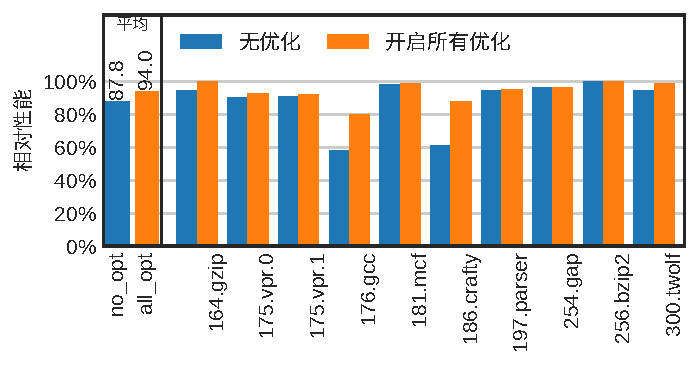
\includegraphics[width=1\linewidth]{./plot_pdf/ucache_ipc.pdf}
%   \caption{微译器运行SPEC CPU 2017的性能,相对于未修改过的X86指令缓存模式进行了归一化。}
%   \label{img:ucache_ipc}
% \end{figure}

% 图\ref{img:new_cache_miss}展示了微译器在X86上SPEC 2017上的每千条指令的未命中次数(MPKI),
% 根据计算,每千条指令的未命中次数和性能之间的皮尔森相关系数为-0.93,说明未命中次数和性能之间存在很强的负相关性。
% 这也说明了微译器的性能主要受到了未命中次数的影响。

% \begin{figure}[!htbp]
%   \centering
%   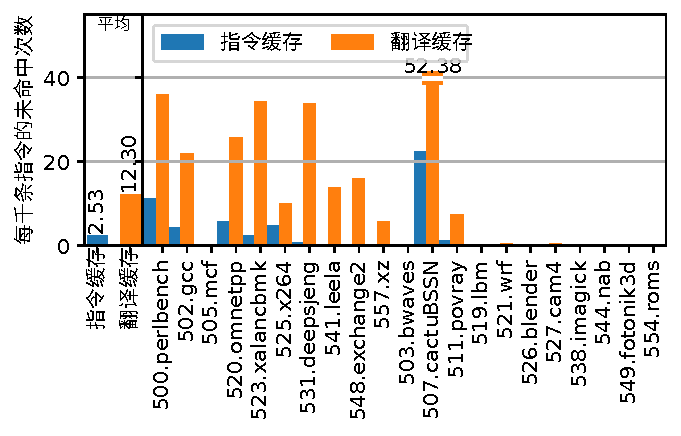
\includegraphics[width=1\linewidth]{./plot_pdf/new_cache_miss.pdf}
%   \caption{微译器运行SPEC CPU 2017的每千条指令的未命中次数。}
%   \label{img:new_cache_miss}
% \end{figure}

% \begin{table}[]
%   \centering
%   \caption{
%     微译器运行CoreMark测试集的性能对比。
%   }
%   \label{tab:coremark}
%   \begin{tabular}{llll}
%   \rowcolor[HTML]{FFCE93} 
%                & x86\_raw & x86\_ucache & riscv\_ucache \\
%   Insts        & 34655642 & 34655642    & 35899262      \\
%   Cycles       & 26220774 & 26301941    & 28797485      \\
%   IPC          & 1.321686 & 1.317608    & 1.246611      \\
%   IPC/IPC\_raw & 100\%    & 99.69\%     & 94.32\%      
%   \end{tabular}
%   \end{table}

% 我们在X86上运行了CoreMark测试集,相对于普通的ICache配置项,也就是没有任何修改的运行X86程序,
% 我们的微译器在翻译运行的性能为99\%,对应的每千条指令的未命中次数为0.9,也符合上述规律,
% 这主要在于程序的取指行为,CoreMark程序中主要为核心循环计算,时间局部性和空间局部性都很好,因此未命中次数较少,性能也较好。
% 即便经过微译器的预翻译文件膨胀,也能够在X86上保持较好的性能。

% 我们在RISCV上运行了CoreMark测试集,得到了性能为94\%,对应的每千条指令的未命中次数为1.1,也符合上述规律。

% RISCV 相对于X86的CoreMark 还有一定的性能差距,主要由于还没有添加硬件返回栈支持,导致对于函数调用的支持不够完善,因此性能有所下降。

% 同时RISCV目前对于压缩指令支持还不够完善,导致翻译出来的微码编码较长,导致AOT文件相对更大,也会导致性能下降。


\section{性能分析}
由于Gem5的模拟器的性能开销较大,我们选择了SPEC CPU 2000 test测试集作为测试基准。
SPEC CPU 2000 test测试集包括了12个整数测试程序和14个浮点测试程序,是一个较为完备的测试集。
目前已经成功运行了8个整数测试程序,剩下的整数测试程序由于指令翻译的问题暂时无法运行,目前还在修复中,浮点测试程序还没有测试。

如图\ref{img:ipc}所示,我们的微译器在运行SPEC CPU 2000 test测试集时(这里只关注RISCV程序),总共有三个测试配置,分别为:
\begin{itemize}
  \item 使用指令缓存(基准参数):CPU没有修改,通过内存层次、多级缓存和指令缓存,硬件译码并运行RISCV程序。
  \item 使用翻译缓存:软件端二进制翻译器把RISCV指令翻译为融合微码,CPU通过内存层次、多级缓存和微码缓存,硬件运行融合微码。
  \item 使用翻译缓存并有所有优化:在上一个配置基础上,开启了所有优化选项,让一行微码行中存储微码指令数目变多了,减少翻译缓存缺失率。
\end{itemize}

我们以指令每周期数(IPC)作为性能指标,IPC越大,性能越好。以指令缓存模式为基准性能,翻译缓存模式的性能为基准性能的百分比,
并分别测量关闭优化以及开启所有优化的性能。
如图\ref{img:ipc}所示,我们的微译器在运行SPEC2000 整数测试集时,性能表现如下:
在不开启任何优化的情况下,性能表现在加上微码缓存后,性能为原生性能87.8\%,其中主要是176.gcc和186.crafty两个测试程序性能下降较多;
这是由于这两个测试程序代码循环较少,时间局部性较差,指令代码较多,导致了大量的缓存缺失;
而对于其他的几个测试程序,性能大多在90\%以上,说明这些程序的时间局部性较好,性能下降较少,微译器的性能表现较好。

在开启所有优化后,性能为原生性能的94\%,性能提升了6\%,说明优化方案的效果较好。
对于176.gcc和186.crafty两个测试程序,性能提升较多,分别为20\%和24\%。
下一小节将对优化方案进行分析。


\begin{figure}[!htbp]
  \centering
  \includegraphics[width=0.8\linewidth]{./plot/ucache_ipc0.pdf}
  \caption{SPEC2000整数性能对比图。}
  \label{img:ipc}
\end{figure}

如图\ref{img:miss_rate}所示,我们的微译器在运行SPEC2000 整数测试集时,翻译缓存缺失率表现如下:
未开启优化时,缓存缺失率平均为2.3\%,其中最高的为gcc和crafty测试程序,缓存缺失率为7.7\%和9.2\%;这与性能表现相符,缓存缺失率越高,性能越低。
开启所有优化后,缓存缺失率平均为0.6\%,下降了1.7\%,说明优化方案的效果较好。
经过计算,缓存缺失率和性能之间的皮尔森相关系数为-0.91,说明缓存缺失率和性能之间存在很强的负相关性。目前的性能下降主要受到了未命中次数的影响。

\begin{figure}[!htbp]
  \centering
  \includegraphics[width=0.8\linewidth]{./plot/miss_rate.pdf}
  \caption{SPEC2000整数测试下缓存缺失率。}
  \label{img:miss_rate}
\end{figure}

如图\ref{img:ipc_fp}所示,我们的微译器在运行SPEC2000 浮点测试集时,性能表现如下:
在不开启任何优化的情况下,性能表现在加上微码缓存后,性能为原生性能的96.5\%;
在开启所有优化后,性能为原生性能98.2\%,性能提升了1.7\%。
这说明无论是否开启优化,微译器对于浮点性能表现较好。


\begin{figure}[!htbp]
  \centering
  \includegraphics[width=0.8\linewidth]{./plot/ucacheipc_fp.pdf}
  \caption{SPEC2000浮点性能对比图。}
  \label{img:ipc_fp}
\end{figure}


\section{优化方案分析}

\begin{figure}[!htbp]
  \centering
  \includegraphics[width=0.8\linewidth]{./plot/ucache_ipc1.pdf}
  \caption{SPEC2000整数性能对比图。}
  \label{img:ipc1}
\end{figure}

\begin{figure}[!htbp]
  \centering
  \includegraphics[width=0.8\linewidth]{./plot/ucache_ipc2.pdf}
  \caption{SPEC2000整数性能对比图。}
  \label{img:ipc2}
\end{figure}

\begin{figure}[!htbp]
  \centering
  \includegraphics[width=0.8\linewidth]{./plot/ucache_ipc3.pdf}
  \caption{SPEC2000整数性能对比图。}
  \label{img:ipc3}
\end{figure}

\begin{figure}[!htbp]
  \centering
  \includegraphics[width=0.8\linewidth]{./plot/ucache_ipc4.pdf}
  \caption{SPEC2000整数性能对比图。}
  \label{img:ipc4}
\end{figure}
\chapter{总结与展望}\label{chap:Conclusion}


\section{总结}
本文发现国产处理器因采用不同指令集而引发的软件适配难题和生态碎片化问题,
这阻碍了国产处理器的发展。二进制翻译技术能够缓解这些问题,
但目前高性能二进制翻译器的性能瓶颈仍然存在,只能达到原生性能的80\%,
且软件优化方案已经比较成熟,难以进一步提升性能,亟需软硬件协同的优化。

本文成功在一种新的二进制翻译系统——x86微译器中添加了对RISC-V架构的支持。
此系统的主要目标是在单一硬件平台上实现多指令集的共存,并尽可能地接近原生执行效率。
本研究的主要工作和贡献包括:

1. 成功设计并实现了RISC-V微译器,包括寄存器映射方案及支持272条通用RISC-V指令的51条微码指令。

2. 对RISC-V微译器进行了性能优化,通过行尾放松、分支放松、可变长行、指令压缩等四种优化策略,降低了微码缓存的缺失率,提升了性能。

在Gem5模拟器中实施的原型系统的实验结果表明,
经过优化的RISC-V微译器在执行SPEC 2000测试集时的平均性能达到了原生程序的96.1\%,
有效地缓解了性能瓶颈,并实现了接近原生程序的运行效率。
微译器的同时支持了x86和RISC-V两种指令集,为多架构二进制翻译提供了一种创新的解决方案。

\section{未来展望}

展望未来,有几个潜在的研究方向可能会进一步提升本文提出的RISC-V微译器的功能和性能:

\begin{enumerate}

\item 丰富测试程序:当前的测试主要依赖于SPEC 2000测试集,未来可以考虑增加更多的真实测试程序,
如数据库、编译器、图像处理程序等,以更全面地评估微译器的性能和适用性。

\item 扩展指令集支持:探索将ARM、LoongArch等其他流行指令集整合进微译器,
以增强其对各类国产处理器的支持,进一步提升系统的通用性和适用性。

\item 微架构优化:进一步研究和优化微译器的内部微架构,如改进翻译缓存的组织形式。
通过增加更多的优化策略,如更高效的指令压缩编码、更精简的缓存行元数据信息等,进一步提升缓存存储效率。
还可以通过添加翻译缓存行的预取机制,进一步降低缓存缺失率,提升性能。

\item 硬件实现验证:将研究成果从模拟环境转移到实际硬件上,
以验证系统在真实硬件下的性能表现以及面积和功耗等方面的指标。

\item 融合微码设计:目前的融合微码还是基于Gem5 x86微码的扩展,
但融合微码的实现会极大影响客户指令的翻译膨胀率,
未来可以考虑设计一种更加通用的融合微码, 需要全面考虑多种指令集的特征,
兼顾指令集编码空间、硬件实现复杂度等多方面因素。

\item 系统态支持:当前的微译器主要支持用户态的二进制翻译,
融合微码也只考虑各个指令集的用户态指令,
未来可以考虑增加对系统态指令的支持,
包括如何高效支持各指令集的控制寄存器、系统调用、内存管理等,
以更好地支持操作系统和关键应用程序的翻译。

\end{enumerate}
% \section{存在的不足}
% 尽管本文的研究取得了初步成果,但也存在一些不足之处,需要在未来的工作中加以解决:

% 1. 长期性能测试缺失:当前的测试主要依赖于标准的基准测试程序,缺少在长期运行和复杂应用环境下的性能数据。

% 2. 生态系统适配性考量:虽然微译器支持多架构,但如何更好地融入现有的软件生态系统,特别是操作系统和关键应用程序的支持,仍需深入研究。

% 通过解决这些问题,未来的研究可以更全面地提升微译器的实用性和市场适应性。
%---------------------------------------------------------------------------%
% main content
%-
%-> Appendix
%-
% \cleardoublepage%
% \appendix% initialize the environment
% \chapter{RISC-V指令翻译表}

下表展示了RISC-V指令翻译到微码指令的对应关系,并按照RISC-V指令类型进行了分类。
其中微码指令分为\textbf{已有微码}和\textbf{新加微码}两种,已有微码指令是原有的Gem5 x86微码指令,新加微码指令是新增的类似RISC-V的微码指令。
我们希望新加微码尽可能少来减少编码空间的占用,因此我们尽量将RISC-V指令翻译成已有微码指令。

能发现大部分以w结尾的RISC-V指令会翻译成新加微码指令,这是由于w结尾的指令为RISC-V64相对于RISC-V32新加的操作32位整数的指令,
而Gem5 x86微码指令中没有对应的32位整数操作指令,因此我们需要新加微码指令来实现这些指令。

\begin{longtable}{lllll}
    \caption{RISCV指令翻译表} \\
    \label{app:RISCV}   \\
    \hline
    分类 & riscv 指令 & 翻译成已有微码 & 翻译成新加微码 \\
    \hline
    \endfirsthead
    
    \multicolumn{4}{c}%
    {{\bfseries \tablename\ \thetable\ 续表}} \\
    \hline
    分类 & riscv 指令 & 翻译成已有微码 & 翻译成新加微码 \\
    \hline
    \endhead
    
    \hline
    \endfoot
    
    \hline
    \endlastfoot
    \hline
    移位                         & sll                              & sllflags                     &                                \\
                               & slli                             & sllflagsimm                  &                                \\
                               & sllw                             &                              & sllw                           \\
                               & slliw                            &                              & sllwimm                        \\
                               & srl                              & srlflags                     &                                \\
                               & srli                             & srlflagsimm                  &                                \\
                               & srlw                             &                              & srlw                           \\
                               & srliw                            &                              & srlwimm                        \\
                               & sra                              & sraflags                     &                                \\
                               & srai                             & sraflagsimm                  &                                \\
                               & sraw                             &                              & sraw                           \\
                               & sraiw                            &                              & srawimm                        \\
                               \hline
    算数                         & add                              & addflags                     &                                \\
                               & addi                             & addflagsimm                  &                                \\
                               & addw                             &                              & addw                           \\
                               & addiw                            &                              & addwimm                        \\
                               & sub                              & subflags                     &                                \\
                               & subw                             &                              & subw                           \\
                               & lui                              & limm                         &                                \\
                               & auipc                            &                              & auipcimm                       \\
                               \hline
    逻辑                         & xor                              & xorflags                     &                                \\
                               & xori                             & xorflagsimm                  &                                \\
                               & or                               & orflags                      &                                \\
                               & ori                              & orflagsimm                   &                                \\
                               & and                              & andflags                     &                                \\
                               & andi                             & andflagsimm                  &                                \\
                               \hline
    比较                         & slt                              &                              & slt                            \\
                               & slti                             &                              & sltimm                         \\
                               & sltu                             &                              & sltu                           \\
                               & sltiu                            &                              & sltuimm                        \\
                               \hline
    分支                       & beq                              &                              &                                \\
                               & bne                              &                              &                                \\
                               & blt                              &                              &                                \\
                              & bge                              & \multirow{-4}{*}{}           & \multirow{-4}{*}{condjumpimm}  \\
                               & bltu                             &                              &                                \\
                              & bgeu                             & \multirow{-2}{*}{}           & \multirow{-2}{*}{condjumpuimm} \\
    \hline
    其他                         & jal                              &                              & jalimm/call            \\
                               & jalr                             &                              & jalrimm/ret                 \\
                               & fence                            & mfence                       &                                \\
                               & fence.i                          & mfence                       &                                \\
                               & ecall                            & syscall                      &                                \\
                               & ebreak                           & syscall                      &                                \\
                               \hline
    乘除法指令                      & mul                              &                              & mul                            \\
                               & mulw                             &                              & mulw                           \\
                               & mulh                             &                              & mulh                           \\
                               & mulhsu                           &                              & mulhsu                         \\
                               & mulhu                            &                              & mulhu                          \\
                               & div                              &                              & div                            \\
                               & divu                             &                              & divu                           \\
                               & divw                             &                              & divw                           \\
                               & divuw                            &                              & divuw                          \\
                               & rem                              &                              & rem                            \\
                               & remu                             &                              & remu                           \\
                               & remw                             &                              & remw                           \\
                               & remuw                            &                              & remuw                          \\
                               \hline
    浮点移动                       & fmv.w.x                          &                              & mov2fpword                     \\
                               & fmv.x.w                          &                              & mov2intword                    \\
                               & fmv.d.x                          & mov2fp                       &                                \\
                               & fmv.x.d                          & mov2int                      &                                \\
                               & fcvt.s.w                         &                              &                                \\
                               & fcvt.d.w                         &                              &                                \\
                               & fcvt.s.wu                        &                              &                                \\
                               & fcvt.d.wu                        &                              &                                \\
                               & fcvt.s.l                         &                              &                                \\
                               & fcvt.d.l                         &                              &                                \\
                               & fcvt.s.lu                        &                              &                                \\
                               \hline
    浮点转换                     & fcvt.d.lu                        & \multirow{-8}{*}{}           & \multirow{-8}{*}{cvtgi2f}      \\
                               & fcvt.w.s                         &                              &                                \\
                               & fcvt.w.d                         &                              &                                \\
                               & fcvt.wu.s                        &                              &                                \\
                               & fcvt.wu.d                        &                              &                                \\
                               & fcvt.l.s                         &                              &                                \\
                               & fcvt.l.d                         &                              &                                \\
                               & fcvt.lu.s                        &                              &                                \\
                               & fcvt.lu.d                        & \multirow{-8}{*}{}           & \multirow{-8}{*}{cvtf2gi}      \\
    \hline
    浮点访存                       & flw                              &                              & lwfp                           \\
                               & fld                              & ldfp                         &                                \\
                               & fsw                              & stfp                         &                                \\
                               & fsd                              & stfp                         &                                \\
                               \hline
    浮点运算                       & fadd.s/d                         & maddf                        &                                \\
                               & fsub.s/d                         & msubf                        &                                \\
                               & fmul.s/d                         & mmulf                        &                                \\
                               & fdiv.s/d                         & mdivf                        &                                \\
                               & fsqrt.s/d                        &                              & msqrtf                         \\
                               \hline
    浮点乘加                       & fmadd.s/d                        & mmaddf                       &                                \\
                               & fmsub.s/d                        & mmsubf                       &                                \\
                               & fnmadd.s/d                       &                              & mnmaddf                        \\
                               & fnmsub.s/d                       &                              & mnmsubf                        \\
                               \hline
    浮点符号                       & fsgnj.s/d                        &                              & fsgnj                          \\
                               & fsgnjn.s/d                       &                              & fsgnjn                         \\
                               & fsgnjx.s/d                       &                              & fsgnjx                         \\
                               \hline
    浮点比较                       & fmin.s/d                         & mminf                        &                                \\
                               & fmax.s/d                         & mmaxf                        &                                \\
                               & feq.s/d                          &                              & mcmpf.eq                       \\
                               & flt.s/d                          &                              & mcmpf.lt                       \\
                               & fle.s/d                          &                              & mcmpf.le                       \\
                               & fclass.s/d                       &                              & fclass                         \\
                               \hline
    原子指令                       & lr.w                             & lw                           &                                \\
                               & sc.w                             & st                           &                                \\
                               & lr.d                             & ld                           &                                \\
                               & sc.d                             & st                           &                                \\
                               & amoswap.w/d                      &                              &                                \\
                               & amoadd.w/d                       &                              &                                \\
                               & amoxor.w/d                       &                              &                                \\
                               & amoand.w/d                       &                              &                                \\
                               & amoor.w/d                        &                              &                                \\
                               & amomin.w/d                       &                              &                                \\
                               & amomax.w/d                       &                              &                                \\
                               & amominu.w/d                      &                              &                                \\
    \multirow{-9}{*}{}         & amomaxu.w/d                      & \multirow{-9}{*}{}           & \multirow{-9}{*}{翻译为多条指令}      \\

\end{longtable}


% \chapter{压缩指令列表}

% \begin{table}[]
    \centering
    \caption{压缩指令列表}
    \label{app:compact_insts}
    \begin{tabular}{|l|l|l|l|}
    \hline
    \multicolumn{1}{|l|}{序号} & \multicolumn{3}{c|}{压缩指令名}                                                        \\ \hline
    \multicolumn{1}{|l|}{}    & \multicolumn{1}{l|}{2操作数} & \multicolumn{1}{l|}{1操作数} & \multicolumn{1}{l|}{0操作数} \\ \hline
    1                        & addflags\_sz8             & dec\_sz4                  & invalid                   \\
    2                        & addflagsimm\_sz8          & dec\_sz8                  & halt                      \\
    3                        & addimm\_sz8               & inc\_sz4                  & ldpop                     \\
    4                        & addwimm\_sz8              & inc\_sz8                  & macroop\_movs1            \\
    5                        & addw\_sz8                 & ld\_stack\_subssz\_sz9    & macroop\_movs2            \\
    6                        & andflags\_sz8             & rdip                      & macroop\_movs4            \\
    7                        & andflagsimm\_sz8          & st\_stack\_subssz\_sz9    & macroop\_movs8            \\
    8                        & auipcimm                  & wripcalli                 & macroop\_stos1            \\
    9                        & jalrimm                   & wripcalli\_call           & macroop\_stos2            \\
    10                       & jalrimm\_T0               & wripi                     & macroop\_stos4            \\
    11                       & jalrimm\_ret              & wripi\_call               & macroop\_stos8            \\
    12                       & limm\_sz4                 & wripi\_ret                & mfence                    \\
    13                       & limm\_sz8                 &                           & nop                       \\
    14                       & mov\_sz4                  &                           & syscall                   \\
    15                       & mov\_sz8                  &                           & stcall                    \\
    16                       & orflags\_sz8              &                           &                           \\
    17                       & sraflagsimm\_sz8          &                           &                           \\
    18                       & srlflagsimm\_sz8          &                           &                           \\
    19                       & sllflagsimm\_sz8          &                           &                           \\
    20                       & stpp\_sz1                 &                           &                           \\
    21                       & stpp\_sz2                 &                           &                           \\
    22                       & stpp\_sz4                 &                           &                           \\
    23                       & stpp\_sz8                 &                           &                           \\
    24                       & subflags\_sz8             &                           &                           \\
    25                       & subw\_sz8                 &                           &                           \\
    26                       & subflagsimm\_sz8          &                           &                           \\
    27                       & wripcallflagsi            &                           &                           \\
    28                       & jalimm                    &                           &                           \\
    29                       & jalimm\_call              &                           &                           \\
    30                       & xorflags\_sz4             &                           &                           \\
    31                       & xorflags\_sz8             &                           &                          \\ \hline
    \end{tabular}
    \end{table}% appendix content
%-
%-> Backmatter: bibliography, glossary, index
%-
\backmatter% initialize the environment
\intotoc*{\cleardoublepage}{\bibname}% add link to toc
\artxifstreq{\artxbib}{bibtex}{% enable bibtex
    \bibliography{Biblio/essay.bib}% bibliography
}{%
    \printbibliography% bibliography
}
%---------------------------------------------------------------------------%
%->> Backmatter
%---------------------------------------------------------------------------%
\chapter[致谢]{致\quad 谢}\chaptermark{致\quad 谢}% syntax: \chapter[目录]{标题}\chaptermark{页眉}
%\thispagestyle{noheaderstyle}% 如果需要移除当前页的页眉
%\pagestyle{noheaderstyle}% 如果需要移除整章的页眉

在论文即将完成之际,回顾研究生三年的生涯,内心许多感慨,在此向所有关心、支持和帮助过我的人表示衷心的感谢!

我要感谢党和国家,我出生农村,家里经济条件受限,在初中阶段一直到本科毕业,
一直都获得过国家的贫困生资助,让我能够顺利完成学业。
感谢党和国家对基层教育和公平性的重视,让我有机会从农村,走到省会城市成都,再到国家首都北京,接受更好的教育。

我要感谢我的母校中国科学院大学,我在此完成了本科和硕士的学业。
本科依托于中国科学院的优质教育资源,
我在此奠定了扎实的数学、物理、计算机基础,
本科的操作系统课程、组成原理课程和体系结构课程都让我对计算机系统有了更深的理解,
促使我选择了计算机系统结构作为硕士的研究方向。
硕士期间在中国科学院计算技术研究所和龙芯中科技术有限公司联合成立的龙芯实验室下,
我有幸参与到二进制翻译系统的分析与优化工作,
我在此获得了很多的知识和经验,也认识了许多优秀的同学和老师。

我要向我的硕士生导师王剑老师表示最诚挚的感谢,王老师在我硕士期间给予了我很多的指导和帮助,
并在我研究方向的选择上给予了很多的建议,让我能够顺利完成硕士学业。
此外我还想感谢课题组的张福新老师,他作为龙芯实验室主任和二进制翻译领域的专家,
在我的研究工作中给予了我很多的建议和指导,让我受益匪浅。

我要向实验室师兄谢本壹博士表示感谢,谢博士在带领我入门二进制翻译领域的过程中给予了我很多的帮助,
和谢博士共同完成的两个课题,也让我在代码调试、实验分析制图和论文写作等方面都得到了很多的锻炼。
我还要感谢实验室的其他师兄师姐们、同学们、学弟学妹们,
特别是李欣宇师兄、燕澄皓同学、张壮壮同学、刘天义师兄、张婷婷师姐、陶思成师弟、吴翔师弟等,
我们共同完成的课题让我学到了很多,也感受到了团队合作的重要性。

我还要感谢我的女朋友袁嘉怡,感谢她在我本科和研究生期间对我的支持和鼓励,
让我多次走出困境,重新振作,她的陪伴让我感到很幸福!
她也让我在学业和生活上都能够做到更好的平衡!

最后我要感谢我的父母,是他们的无私付出和默默陪伴,让我能走到今天,他们是我永远的依靠和榜样!

忠心感谢所有关心、支持和帮助过我的人,谢谢你们!

\rightline{2024年6月}
\chapter{作者简历及攻读学位期间发表的学术论文与其他相关学术成果}

\section*{作者简历:}
晏悦,四川成都人,1998年出生。

2017年09月——2021年06月,在中国科学院大学计算机科学与技术学院获得学士学位。

2021年09月——2024年06月,在中国科学院计算技术研究所攻读硕士学位。

\section*{已发表(或正式接受)的学术论文:}

{
\setlist[enumerate]{}% restore default behavior
\begin{enumerate}[nosep]
    \item Xie, Benyi, Xinyu Li, \textbf{Yue Yan}, Chenghao Yan, Tianyi Liu, Tingting Zhang, Chao
    Yang and Fuxin Zhang. “On-Demand Triggered Memory Management Unit
    in Dynamic Binary Translator.”Advanced Parallel Programming Technologies
    (2023).

    \item Xie, Benyi, \textbf{Yue Yan}, Chenghao Yan, Sicheng Tao, Zhuangzhuang Zhang, Xinyu
    Li, Yanzhi Lan, Xiang Wu, Tianyi Liu, Tingting Zhang and Fuxin Zhang.
    “An Instruction Inflation Analyzing Framework for Dynamic Binary Translators.”ACM
    Transactions on Architecture and Code Optimization (2024).
    % \item 已发表的工作2
\end{enumerate}
}


\section*{参加的研究项目:}
\begin{enumerate}[nosep]
    \item 二进制翻译膨胀分析工作\ 合作参与者
    \item x86微译器项目\ 合作参与者
    \item RISC-V微译器项目\ 负责人
\end{enumerate}


\section*{获奖情况:}
\begin{enumerate}[nosep]
    \item 2023年\ 中国科学院计算技术研究所\ 所长优秀奖
    \item 2023年\ 中国科学院大学\ 三好学生
    \item 2023年\ 龙芯中科技术有限公司\ 龙芯实验室优秀学生
\end{enumerate}

\cleardoublepage[plain]% 让文档总是结束于偶数页,可根据需要设定页眉页脚样式,如 [noheaderstyle]
%---------------------------------------------------------------------------%
% other information
\end{document}
%---------------------------------------------------------------------------%

